\chapter{Literature Review}
\label{cap:Literature}

This chapter explores the multifaceted world of  translation. We start by examining translation as intercultural communication, exploring challenges like achieving equivalence in meaning and the unique demands of subtitling. We then address the limitations of human translation and the rise of technological solutions, like NMT systems and LLMs. Next, we focus on the specific challenge of translating spatial language, exploring spatial semantics (categories, patterns), the intricacies of English spatial prepositions, and the difficulties that arise when translating them between EN-PT-br. Finally, we conclude by examining methods for assessing translation quality, including human evaluation, manual error classification for spatial semantics, and automatic evaluation metrics.


\section{Translation as Intercultural Communication}

\epigraph{A language is not just words. It’s a culture, a tradition, a unification of a community, a whole history that creates what a community is. It’s all embodied in a language. \\ \hfill --- Noam Chomsky}

In our increasingly interconnected world, overcoming language barriers is crucial for fostering understanding and connection across cultures. Translation, the process of converting text from one language (source) to another (target), plays a vital role in this cross-cultural exchange. As noted by~\textcite[p. 9-10]{house2018}, it allows individuals from diverse backgrounds to access knowledge and experiences beyond their linguistic borders, enriching their understanding of the world through different perspectives.

However, translation goes beyond simply transfering linguistic content from a source text to a target text. It entails a series of complex cognitive processes that happens within the translator's brain, as well as a deep understanding of cultural interplay, as language, cognition, and culture are intricately linked. According to~\textcite{house2014translation}, every word and phrase carries not just its literal meaning but also cultural context, shaping how we view the world. This quote, from her book \enquote{Translation Quality Assessment: Past and present}, underscores the complex interplay between language, culture, and cognition in translation.


\begin{quote}
Language is culturally embedded: it serves to express and shape cultural reality, and the meanings of linguistic units can only be understood when considered together with the cultural contexts in which they arise, and in which they are used. In translation, therefore, not only two languages but also two cultures invariably come into contact. In this sense, then, translation is a form of intercultural communication. Over and above recognizing the importance of the two larger macro-cultural frameworks, however, the translator must of course also consider the more immediate ‘context of situation’. This more local situational context has to do with questions about who wrote the text, when, why, for whom, and who is now reading it, and for what purpose, etc. These questions, in turn, are reflected in how a text is written, interpreted, read and used. The context of situation is itself embedded in the larger socio-cultural world as it is depicted in the text and in the real world. \\
\phantom{abc} \hfill --- \textcite[4]{house2014translation}
\end{quote}

In that sense, translating effectively, as highlighted by~\textcite{house2014translation}, extends beyond conveying factual content. Translators navigate a challenging landscape, acting as bridges not only between languages but also the cultural contexts they embody. Beyond linguistic proficiency, they require critical situational judgment to understand the social and cultural environments of both source and target audiences. This balancing act demands ensuring the target text accurately reflects the intended meaning of the source language while faithfully representing its original message and cultural nuances~\parencite{house2018}. 

Achieving this balance becomes even more crucial in the current information age, marked by rapid technological advancements. While globalization has increased translation demand, it also intensifies the challenges of instant information flow and its reliance on English as a global lingua franca. The dominance of English, as noted by~\textcite[4]{house2014translation}, raises concerns about potential harm to language diversity and the diminished representation of diverse cultures in the global information flow.


\subsection{Translation and Equivalence}

Building upon the understanding that translation involves both cognitive processes and socio-cultural awareness, the concept of equivalence becomes crucial for achieving effective communication across cultures. 

While a literal translation might seem straightforward, it often falls short due to inherent differences between languages. \enquote{Equivalence}, unlike sameness or identity, focuses on conveying meaning with roughly equal value across these differences. Its Latin origin, meaning \enquote{of equal value,} emphasizes this core principle: acknowledging and working with the unavoidable differences between languages. As ~\textcite[6]{house2014translation} points out, this means preserving the intended meaning across different cultures.

\begin{quote}
The notion of equivalence is also related to the preservation of \enquote{meaning} across two different lingua-cultures. Three aspects of that meaning are particularly relevant for translation: a semantic aspect, a pragmatic aspect and a textual aspect. \\
\phantom{abc} \hfill --- \textcite[21]{house2014translation}
\end{quote}


The \textit{semantic meaning}, as explained by the author, focuses on the designated sense of words and their connection to the objects or ideas they represent. In contrast, \textit{pragmatic meaning} extends beyond the word level to include the speaker's intent, the communication context, and the impact on the listener. \textcite{house2014translation} highlights that pragmatic meaning emerges from the interaction between language, the speaker’s intention, the context, and the listener, contributing to the overall meaning-making process within a social setting.

The translation scholar further emphasizes this distinction by referencing a theorical work that helps us understand how utterances function beyond simply conveying information. The theory proposed by~\textcite{austin1962how, Searle1995-SEATCO}, known as speech act theory, introduces the concept of ``illocutionary force'', which essentially refers to the specific purpose or function of an expression in a particular context. This is distinct from the propositional content, which is the literal information conveyed. While grammatical features sometimes hint at the illocutionary force, \textcite[22]{house2014translation} clarifies that the context ultimately plays a crucial role in determining it in real-world situations.

Because translation deals with language in use, according to~\textcite[22]{house2014translation}, understanding the intended meaning and impact of a statement is crucial. Unlike dictionaries, for instance, which deal with isolated word meanings, translators work with complete units of communication (utterances) used in real-world situations. This means they consider not just the literal meaning of words (semantic meaning) but also the speaker's intent, the context, and the desired effect on the listener (pragmatic meaning). The author acknowledges that, sometimes, prioritizing the intended message and impact might require sacrificing some degree of literal meaning. Imagine trying to translate a joke – focusing solely on word-for-word accuracy might miss the humor entirely. In such cases, the translator aims for functional equivalence, ensuring the translated message conveys the original intent and effect even if the wording differs slightly.

Finally, the last aspect, \textit{textual meaning}, is another crucial element for achieving equivalence in translation, as emphasized by~\textcite[22-23]{house2014translation}. A text, the author explains, is any stretch of language where its individual components are interconnected and form a cohesive whole. Think of it like a paragraph or longer passage where sentences work together to convey a larger meaning. Various relationships within the text, such as theme progressions, pronouns, substitutions, and references, contribute to the overall textual meaning that needs to be considered during translation \parencite{house2014translation}.

With that in mind, achieving effective cross-cultural communication through translation necessitates a nuanced approach that goes beyond simply matching words from one language to another. Equivalence, acknowledging and working with the inherent differences between languages, is key to preserving the intended meaning across cultures. As we move forward, understanding the complexities of equivalence will remain central to fostering effective communication in our increasingly interconnected world.


\subsection{Subtitling and its Unique Challenges}

The global landscape of entertainment has shifted dramatically. The rise of streaming platforms have fueled a surge in demand for accessible multilingual content. Movies, TV shows, documentaries, and other audiovisual media are now translated into numerous languages to cater to diverse audiences. This abundance of translated content highlights the critical importance of providing accurate and culturally nuanced translations.

In this context, \emph{subtitling}, the process of displaying translated text synced with the audio, plays an important role. It fosters cultural exchange by allowing non-native speakers to access and understand foreign media. However, subtitling presents a unique set of challenges distinct from traditional written translation. As translation scholars \textcite{cintas2020subtitling} point out, subtitling goes beyond simply translating spoken words. It encompasses various elements of the audiovisual experience:

\begin{quote}
(Subtitling) may be defined as a translation practice that consists in presenting a written text, generally on the lower part of the screen, that aims to recount the original dialogue exchanged among the various speakers, as well as all the other verbal information that is transmitted visually (letters, inserts, graffiti, text messages, inscriptions, placards, and the like) and orally (songs, voices of, voiceover narration). \\
\phantom{abc} \hfill --- \textcite[9]{cintas2020subtitling}
\end{quote}

This multifaceted nature, as highlighted above, presents unique challenges distinct from traditional written translation, as \textcite{cintas2020subtitling} further explain:

\begin{quote}
All subtitled programmes are made up of three main constituents: the spoken word, the image and the subtitles. The interaction of these three components, along with the viewer’s ability to read both the images and the written text at a particular speed, and the actual size of the screen, determine the basic characteristics of the audiovisual medium. Subtitles must appear in synchrony with the images and dialogue, provide a semantically adequate account of the SL (source language) dialogues, and remain displayed on screen long enough for the viewers to be able to read them. \\
\phantom{abc}
\hfill --- \textcite[9]{cintas2020subtitling}
\end{quote}

These complexities, as outlined in the second quote, contribute to the specific challenges faced by subtitlers. Unlike written text, subtitles are constrained by limited space and the need to synchronize with both the speaker's pace and the viewer's reading speed. Additionally, conveying cultural references and technical vocabulary within these time constraints demands creative solutions~\parencite{matusov-etal-2019-customizing}. Subtitlers must therefore possess a diverse skill set, including proficiency in both languages, excellent writing skills, cultural sensitivity, and the ability to condense meaning while maintaining clarity and accuracy~\parencite{cintas2020subtitling}.

In this master's thesis research, due to time constraints, we will treat the segments in our subtitle corpus as complete spoken utterances. This approach temporarily sets aside the limitations inherent to subtitling, such as screen time limits and character restrictions. For example, consider a complex spatial expression conveyed in a long sentence, such as ``The bird flew down from out of the hole in the tree and onto the little girl's face as she walked along the sidewalk. '' In subtitling, this sentence might be split into multiple lines due to character limits, potentially losing the nuances and complexity of the original expression. By simplifying the analysis in this way, we focus on investigating the linguistic phenomenon at hand and establish a foundation for further research, which will allow us to address subtitling constraints in future studies.


\subsection{Human Translation: Current Limitations and the Need for Technological Solutions}

Throughout history, human translation has been pivotal in various aspects of human development. It has facilitated the invention and spread of writing systems, fostered the formation of national languages and literatures, and enabled the exchange of knowledge, political power, and cultural influences across borders. According to \textcite{house2014translation}, human translation has been invaluable in various domains, from diplomatic negotiations to scientific collaborations and the dissemination of religions and cultural values.

Even in the modern world, human translators' deep cultural and linguistic knowledge uniquely equips them to capture the nuances, cultural references, idioms, and context of the source language, enabling them to deliver high-quality translations ~\parencite{dalayli-2023-use}.

Nevertheless, human translation faces challenges in \emph{scalability}. Individual limitations in capacity and time, coupled with the often-necessary research to ensure the quality of the traslated texts, can hinder its effectiveness in large-scale projects. As highlighted by \textcite{kenny2022human} in her paper ``Human and Machine Translation,'' time-consuming research is frequently needed when translators encounter difficulties understanding the source text, recalling specific terminology, or formulating ideas in the target language:

\begin{quote}
When a professional translator does not understand something in the source text, or cannot recall a specialized term in the target language, or is struggling to come up with a way of formulating an idea in the target language, she will usually divert her attention from the text at hand, and do some research. A translator grappling with the niceties of wastewater treatment, for example, may go to the website of various local authorities to see how they explain the technology involved. She might access one of the many publicly available termbanks to find an equivalent for a given term. She might consult other documentation produced by her client’s company or speak to engineers at the company. \\
\phantom{abc} 
\hfill --- \textcite[29]{kenny2022human}
\end{quote}

This research-intensive process, while crucial for maintaining translation quality, emphasizes the scalability limitations of human translation. As \textcite{kenny2022human} further details, translators may encounter specialized fields or poorly written source texts requiring additional effort and expertise beyond their immediate domain:

\begin{quote}
Even experienced translators will sometimes admit to difficulty in translating texts that are highly technical and for which they lack sufficient training. Whereas a translator with an educational or professional background in legal studies or practice might relish working on the translation of legislation, a specialist in automotive engineering will run (or drive) a mile from such work. It can also happen that, even within their own domain, translators can come across source texts that are badly written, or incomplete, or written in a way that makes them extremely difficult to understand. \\
\phantom{abc}
\hfill --- \textcite[29]{kenny2022human}
\end{quote}

While specialization equips translators to handle complex texts, it necessitates constant upskilling and increases \emph{costs}, further hindering scalability, particularly for smaller projects where human translation is cost-prohibitive. These limitations pave the way for the exploration of technological solutions alongside human expertise. As a result, MT has emerged as a powerful tool, widely adopted across various translation fields, due to its suitability for large-scale applications and cost-effectiveness for specific content types  \parencite{karakanta-etal-2020-42}. As emphasized by \textcite{kenny2022human}:

\begin{quote}
The use of MT in translation production does not necessarily entail a loss of quality, and the cost and effort of human translation is not appropriate for all types of texts, particularly those with a short shelf-life that present little risk. \\
\phantom{abc} \hfill --- \textcite[129-130]{kenny2022human}
\end{quote}

For \textcite{kenny2022human}, the use of MT can be particularly beneficial in scenarios where human translation costs or turnaround times are limited. This supports the notion that MT is not meant to replace human translators entirely, but rather complement their expertise in situations where its strengths are best suited. That said, it is important to acknowledge that MT is still under development. Its ability to handle the complexities of audiovisual translation (AVT) and creative texts, for instance, remains limited due to the inherent challenges in understanding these specific content types \parencite{Burchardt2016}.

Therefore, in the quest for effective translation solutions, a hybrid approach that combines the strengths of both human and machine translation is gaining prominence. By leveraging human expertise for tasks requiring creativity, cultural understanding, and domain-specific knowledge, and utilizing MT for routine or large-scale projects, this hybrid approach achieves both scalability and cost-effectiveness while preserving quality.

This evolving landscape requires adaptation from practicing translators. Their roles are transforming towards \emph{post-editing} tasks, as highlighted by Robert Lane Greene in The Economist's Technology Quarterly on Language:

\begin{quote}
The ‘translator’ of the future is likely to be more like a quality control expert, deciding which texts need the most attention to detail and editing the output of MT software. That may be necessary because computers, no matter how sophisticated they have become, cannot yet truly grasp what a text means.\\
\phantom{abc} \hfill --- \textcite{economist2017}
\end{quote}

All in all, despite its historical importance, human translation faces limitations in scalability and cost in the modern world, necessitating alternative solutions. While MT offers advantages in these areas, its ongoing development means it struggles with complexities like audiovisual translation and creative texts. The future, therefore, lies in a collaborative approach, where human expertise tackles nuances and complexities while MT handles routine tasks. This synergy between humans and machines paves the way for efficient, cost-effective, and high-quality translations, fostering communication across languages in a globalized world.


\section{Translating Spatial Language}
\label{sec: translating-spatial}

\epigraph{Language is not just a tool for communication; it is also a tool for thought. Our language shapes the way we think and the ideas we can conceive. \\ \hfill --- George Lakoff}

The study of spatial expressions, that is, the diverse ways through which we use language to convey motion, location, and spatial relationships between objects, has become a significant field of research across various disciplines \parencite{levinson2006grammars}. This growing interest stems from the crucial role spatial language play in diverse fields like Cognitive Linguistics~\parencite{LakoffJohnson80, talmy1985lexicalization, talmy2000toward, talmy2000towardb, oliveira2022expressing}, Cognitive Psychology~\parencite{slobin1985crosslinguistic, slobin1987thinking, slobin1996thought, slobin2005relating, taylor1996perspective,  tversky2003structures, oliveira2021hipotese}, Semantics~\parencite{zwarts2016counterdirectionality}, Natural Language Processing~\parencite{dobnik2018exploring, ghanimifard2019neural, kelleher2022distributional}, and Artificial Intelligence~\parencite{gotts1996connection, ligozat2007language, zang2018translating, rodrigues2017pinning, rodrigues2020standpoint}.

Despite its undeniable importance, defining the exact scope of spatial language remains a multifaceted challenge due to its interdisciplinary nature. \textcite{zlatev-spatial} emphasizes that the spatial domain is not easily delineated and often overlaps with other types of meaning, complicating efforts to establish clear boundaries. Furthermore, in Cognitive Linguistics, space is frequently used metaphorically to represent abstract concepts, such as time (e.g., ``I'll arrive \emph{on} time''), emotions (e.g., ``She's \emph{in} love''), and idiomatic expressions (e.g., ``He's feeling \emph{under} the weather'') \parencite{ coventry:04b}. This metaphorical use of space reflects how spatial relationships extend beyond physical dimensions to encompass how humans conceptualize and organize abstract ideas based on their bodily experiences. Thus, space functions both as a literal and metaphorical framework, influencing how we understand and convey spatial relationships and concepts.

However, despite these complexities, this section aims to explore the nuances involved in translating spatial expressions for the EN-PT-br pair. We will examine how different parts of speech lexicalize spatial meanings in the two languages, before ultimately focusing our attention on prepositions ACROSS, THROUGH, INTO, and ONTO.


\subsection{Spatial Semantics: Categories and Lexicalization Patterns} 

This section explores the complexities involved in translating ``Motion Events'' across languages. While numerous fundamental categories have been proposed in the literature, a comprehensive analysis can be a challenging task. Therefore, this study adopts the semantic concepts of \emph{Figure}, \emph{Ground}, \emph{Motion}, \emph{Path}, \emph{Manner}, and \emph{Cause} \parencite{talmy1985lexicalization, talmy2000toward, talmy2000towardb}. These terms, though not all universally adopted, align well with our chosen approach, despite minor variations in different research perspectives.


\subsubsection{The Semantic Components of Motion Events} 

The basic ``Motion event'', as defined by \textcite[25-26]{talmy2000towardb}, involves a single object (the Figure) located or moving relative to another object (the reference object, or Ground) in either \emph{self-contained} or \emph{translational motion}. The first type refers to motion without a change of location in space, such as rotation, oscillation, or dilation, while the latter involves the Figure’s location changing over time \parencite{shan2018review}. This concept is broken down into four essential components: 

\begin{itemize}
  \item \emph{Figure} (F): The object moving or in static location.
  \item \emph{Ground} (G): The reference object serving as a point of comparison.
  \item \emph{Path} (P): The path taken by the Figure in relation to the Ground (when moving) or its fixed location (when static).
  \item \emph{Motion}: The state of the Figure --- either moving (MOVE) or stationary (BE\begin{scriptsize}LOC\end{scriptsize}).
\end{itemize}

In addition to the four core components, Motion events can be accompanied by an external element called ``Co-event'', typically expressing the Manner (M) and/or Cause (C) of the motion. These additional elements, as well as the essential four described above, can be observed in Examples~\ref{ex:2}, \ref{ex:3}, \ref{ex:4}, and \ref{ex:5} adapted from \textcite{talmy2000towardb}. 
Figure~\ref{fig:patterns-events} summarizes the semantic schema of Motion events.

\footnotesize{
\ex. MOVE + Manner: \label{ex:2}
    \a. The rock\begin{scriptsize}$<$F$>$\end{scriptsize} \textbf{rolled}\begin{scriptsize}$<$MOVE + M$>$\end{scriptsize} \textit{down}\begin{scriptsize}$<$P$>$\end{scriptsize} the hill\begin{scriptsize}$<$G$>$\end{scriptsize}. $=$ 
    [the rock MOVED down the hill] WITH-THE-MANNER-OF [the rock rolled] 
    \b. The gate\begin{scriptsize}$<$F$>$\end{scriptsize} \textbf{swung}\begin{scriptsize}$<$MOVE + M$>$\end{scriptsize} shut \textit{on}\begin{scriptsize}$<$P$>$\end{scriptsize} its rusty hinges\begin{scriptsize}$<$G$>$\end{scriptsize}. $=$ [the gate MOVED shut ($=$ the gate shut)] WITH-THE-MANNER-OF [the gate swung on its rusty hinges] 

\ex. MOVE + Cause: \label{ex:3}
    \a. The napkin\begin{scriptsize}$<$F$>$\end{scriptsize} \textbf{blew}\begin{scriptsize}$<$MOVE + C$>$\end{scriptsize} \textit{off}\begin{scriptsize}$<$P$>$\end{scriptsize} the table\begin{scriptsize}$<$G$>$\end{scriptsize}. $=$ 
    [the napkin MOVED off the table] WITH-THE-CAUSE-OF [(something) blew on the napkin] 
    \b. The man \textbf{hammered}\begin{scriptsize}$<$MOVE + C$>$\end{scriptsize} the nail\begin{scriptsize}$<$F$>$\end{scriptsize}  \textit{into}\begin{scriptsize}$<$P$>$\end{scriptsize} the board\begin{scriptsize}$<$G$>$\end{scriptsize} with a mallet. $=$ [the man MOVED the nail into the board] WITH-THE-CAUSE-OF [he hammered it with a mallet] 
    
\ex. BE\begin{scriptsize}LOC\end{scriptsize} + Manner: \label{ex:4}
    \a. The lamp\begin{scriptsize}$<$F$>$\end{scriptsize} \textbf{stood}\begin{scriptsize}$<$BE\begin{scriptsize}LOC\end{scriptsize} + M$>$\end{scriptsize} \textit{on}\begin{scriptsize}$<$P$>$\end{scriptsize} the table\begin{scriptsize}$<$G$>$\end{scriptsize}. $=$ [the lamp BE\begin{scriptsize}LOC\end{scriptsize} on the table] WITH-THE-MANNER-OF [it stood there]
    \b. The rope\begin{scriptsize}$<$F$>$\end{scriptsize} \textbf{hung}\begin{scriptsize}$<$BE\begin{scriptsize}LOC\end{scriptsize} + M$>$\end{scriptsize} \textit{across}\begin{scriptsize}$<$P$>$\end{scriptsize} the canyon\begin{scriptsize}$<$G$>$\end{scriptsize} from two hooks. $=$ [the rope BE\begin{scriptsize}LOC\end{scriptsize} across the cannyon] WITH-THE-MANNER-OF [it hung there]

\ex. BE\begin{scriptsize}LOC\end{scriptsize} + Cause: \label{ex:5}
    \a. The pencil\begin{scriptsize}$<$F$>$\end{scriptsize} \textbf{stuck}\begin{scriptsize}$<$BE\begin{scriptsize}LOC\end{scriptsize} + M$>$\end{scriptsize} \textit{on}\begin{scriptsize}$<$P$>$\end{scriptsize} the table\begin{scriptsize}$<$G$>$\end{scriptsize} (after I glued it). $=$ [the pencil BE\begin{scriptsize}LOC\end{scriptsize} on the table] WITH-THE-MANNER-OF [it stuck there (after I glued it)]


\normalsize{

\begin{figure}[htb]
\centering
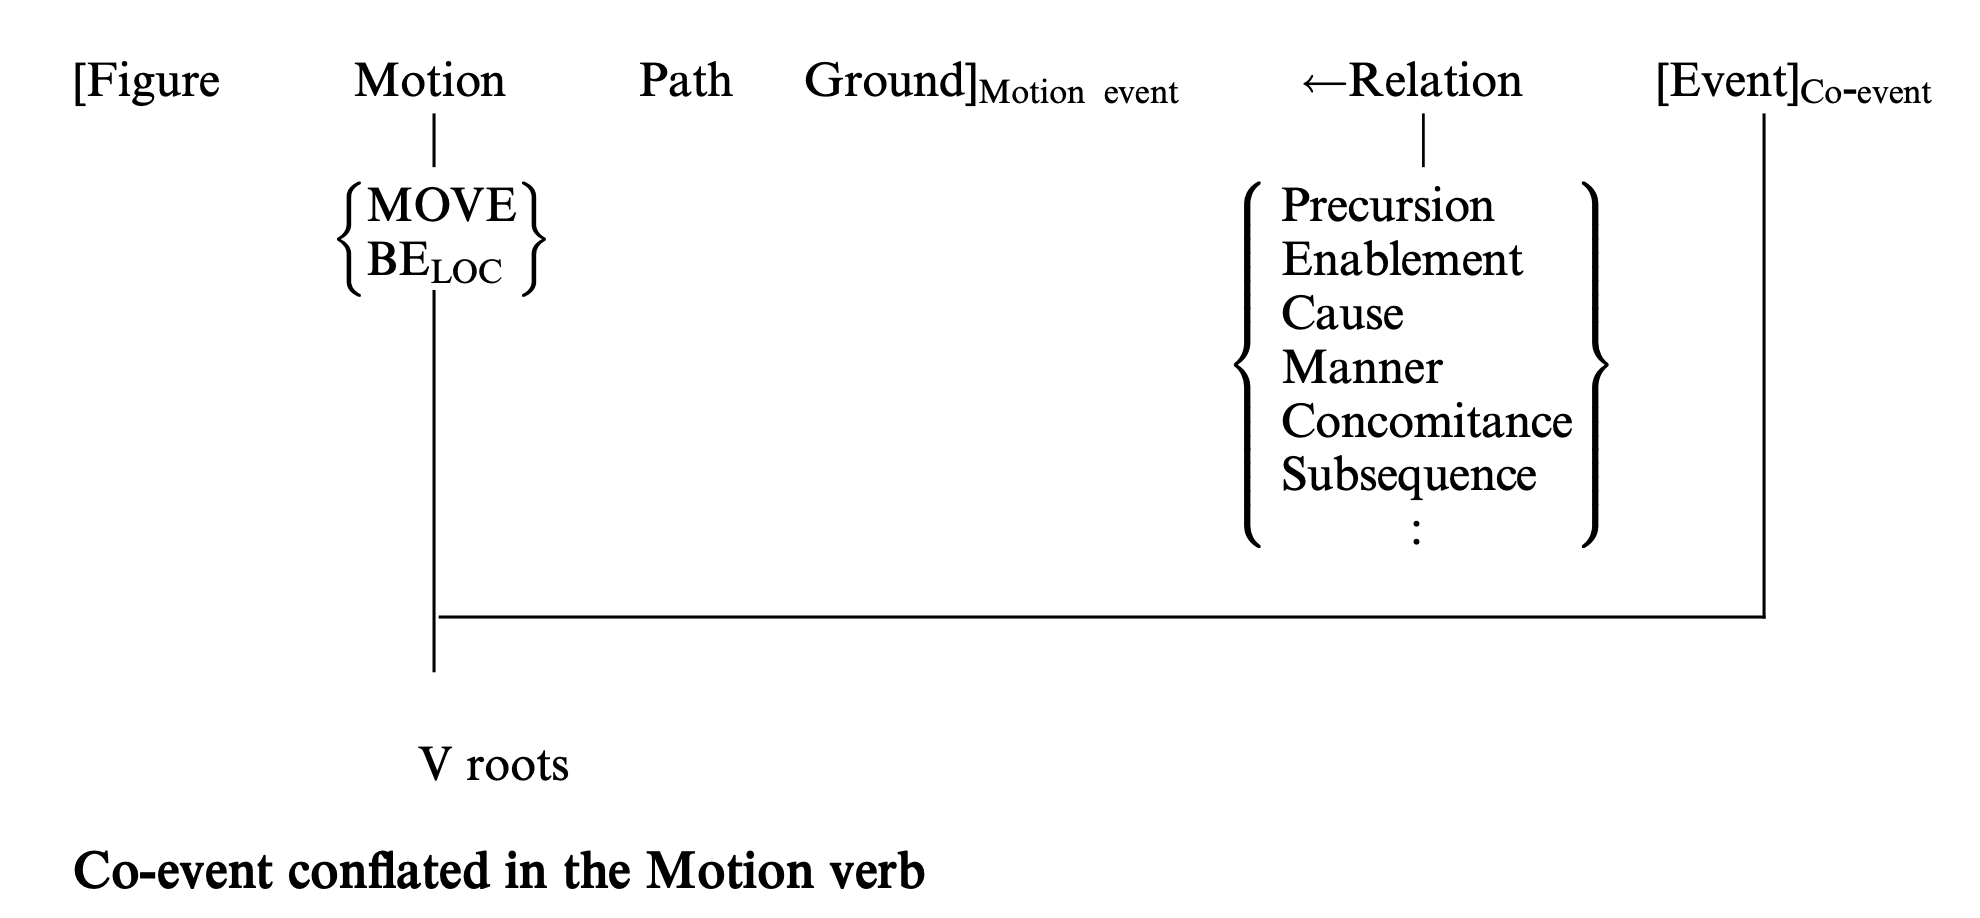
\includegraphics[width=0.8\textwidth]{figuras/Screen Shot 2024-05-17 at 13.01.00.png}
\caption{\label{fig:patterns-events} Patterns in Representation of Event Structure  \parencite[28]{talmy2000towardb}.}
\end{figure}


\subsubsection{Meaning and Form in Language}

\textcite[21]{talmy2000towardb} argues for a systematic connection between \textit{meaning} and \textit{form} in language. Semantic concepts (like \emph{Figure}, \emph{Ground} and \emph{Motion}) represent the linguistic meanings. Surface expressions, on the other hand, represent the various grammatical forms used to convey these meanings, such as verbs, adpositions, subordinate clauses, and \emph{satellites}. The latter are defined as closed-class elements like prepositions and adverbials that have a ``sister relation" to verbs and other phrases \parencite{oliveira2022expressing}.
 
\begin{quote}
A combination of semantic elements can be expressed by a single surface element, or a single semantic element by a combination of surface elements. Or again, semantic elements of different types can be expressed by the same type of surface element, as well as the same type by several different ones. We find here a range of universal principles and typological patterns as well as forms of diachronic category shift or maintenance across the typological patterns. \\
\phantom{abc}
\hfill --- \textcite{talmy2000towardb}
\end{quote}

Understanding this intricate relationship between meaning and form is crucial for an accurate translation. \textcite{talmy2000towardb}'s observation highlights the multifaceted nature of this connection. A single semantic element, like Manner, can be conveyed through various surface forms depending on the language (e.g. the verb ``to struggle'' in English can be expressed by ``debater-se'' (to flounder), ``tentar duramente'' (try hard)  ou ``fazer um grande esforço'' (make a big effort) in Portuguese, that is, through a verb, a verb-adverb combination, or even a complex clause). Conversely, the same surface form in one language might encode different semantic elements in another. For instance, the English preposition ``into,'' used to convey the Path element with directionality, might require a combination of surface forms like ``entrar em/dentro de'' (go into) in Portuguese.

However, it is important to recognize that even skilled human translators may not always have explicit linguistic awareness of these nuances. High-quality translation often relies on an intuitive grasp of language and context rather than a detailed, conscious understanding of linguistic theory. Therefore, while translators may effectively handle these challenges in practice, the theoretical complexity of meaning and form highlights the importance of developing and refining automated translation systems to bridge potential gaps in linguistic knowledge and achieve more nuanced and accurate translations.

\subsubsection{The Spatial Domain: from Language Typology to Neo-determinism}

Based on a systematic observation of universal and typological features across human languages, \textcite{talmy2000towardb} proposes a two-fold typological classification of language groups. The first group, \texttt{satellite-framed} languages, primarily express Motion and Co-events (Cause or Manner) through a single verb root (e.g., to run, to crawl, to climb). They also have a smaller set of verbs to express static location with these additional elements. The Path component, on the other hand, is generally expressed in a satellite (e.g. prepositions). English, as well as other Germanic languages, such as German and Dutch, and most Indo-European languages (except Romance) are a part of this group. 

In contrast, \texttt{verb-framed} languages typically separate Motion from Co-events. Their verbs primarily encode the Path element (e.g., enter, pass, exit), while Manner or Cause are expressed with separate words like adverbs, gerunds, or prepositional phrases. Romance languages like Portuguese and Spanish, Semitic languages, Basque, Korean, and Japanese fall into this category. Figure~\ref{fig:s-v-distinction} visually summarizes this distinction, and Examples~\ref{ex:5a} and~\ref{ex:5b} from \textcite{oliveira2022expressing}, further illustrate the two groups.

\begin{figure}[htb]
\centering
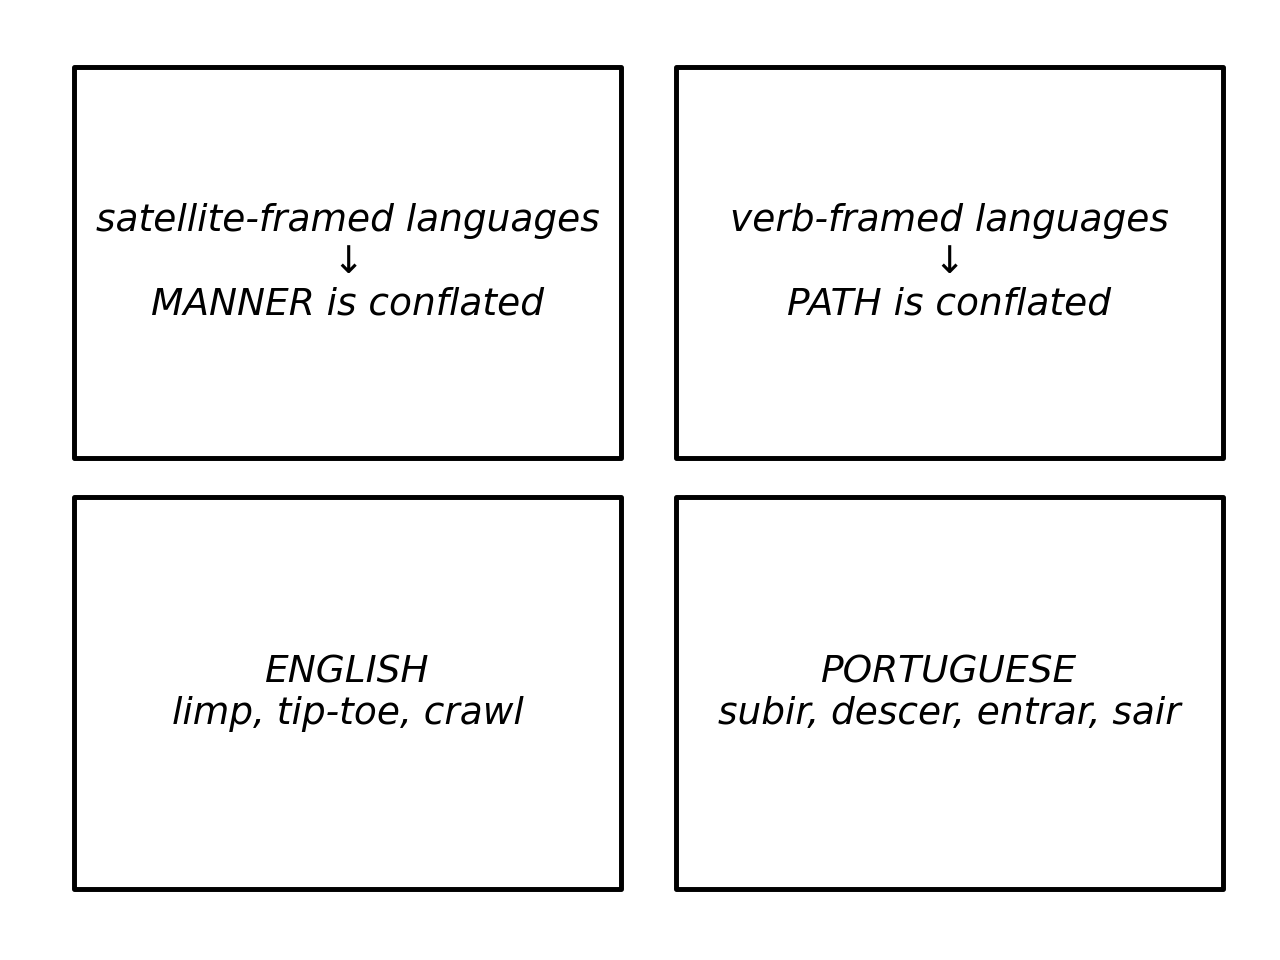
\includegraphics[width=0.7\textwidth]{figuras/Unknown-4.png}
\caption{\label{fig:s-v-distinction} Distinction between English (\texttt{satellite-framed}) and Portuguese (\texttt{verb-framed}) (Source: our own).}
\end{figure}

\ex. 
    \a. The pencil \textbf{rolled}\begin{scriptsize}$<$M$>$\end{scriptsize} \textit{off}\begin{scriptsize}$<$P$>$\end{scriptsize} the table. \\
    \emph{O lápis \textit{saiu}}\begin{scriptsize}$<$P$>$\end{scriptsize} \textbf{\emph{rolando}}\begin{scriptsize}$<$M$>$\end{scriptsize} (e caiu) \emph{da mesa}. \label{ex:5a} 
    \b. The boy \textbf{stepped}\begin{scriptsize}$<$M$>$\end{scriptsize} \emph{aside}\begin{scriptsize}$<$P$>$\end{scriptsize}. \\
    \emph{O garoto se \textit{afastou}}\begin{scriptsize}$<$P$>$\end{scriptsize}. \label{ex:5b}

Interestingly, English commonly uses multiple prepositions to indicate the \emph{trajectory} (or complex path) of a Figure in motion. As \textcite{oliveira2022expressing} point out, this is also why it is very common to find descriptions containing multiple prepositions that indicate the subgoals of a Figure, as shown in Example~\ref{ex:6}.

\ex. 
    The frog \textbf{crawled} \textit{out of} the jar\begin{scriptsize}$<$1$>$\end{scriptsize} and \textit{through} the window\begin{scriptsize}$<$2$>$\end{scriptsize} \textit{into} the woods\begin{scriptsize}$<$3$>$\end{scriptsize}. \label{ex:6} 
    \emph{O sapo escapou} \textbf{sorrateiramente} \emph{da jarra, saiu pela janela e fugiu para a floresta.}


The translation of Example~\ref{ex:6}  illustrates a challenging real-world scenario where the translator prioritizes idiomacity in the target language over original semantic nuances. For instance, ``crawled out of'' is translated as ``escapou sorrateiramente'' (slyly escaped), shifting the focus from the Manner of motion to the outcome of escaping. A more literal translation, such as ``o sapo rastejou para fora,'' would preserve the Manner aspect but would sound less idiomatic in Portuguese. Similarly, ``through the window'' and ``into the woods'' are translated as ``saiu pela janela' and ``fugiu para a floresta,'' emphasizing \emph{changes of state} rather than motion dynamics. In \texttt{verb-framed} languages, such as Portuguese, Manner verbs like ``crawl'' are generally avoided when describing events that involve crossing boundaries due to a ``boundary-crossing constraint,'' where the main verb typically encodes the change of state rather than the activity (Manner of motion), as described by~\textcite{Slobin2006WhatMM}. Exceptions include high-energy, punctual acts that can be conceptualized as a change of state, like ``throw oneself,'' but generally, Manner verbs are incompatible with describing activities extended in time or space across boundaries.

These typological differences raise intriguing questions about the relationship between language and thought. Does language merely reflect our conceptualization of the world, or does it play a more active role in shaping it? This line of inquiry delves into the realm of neo-determinism, which builds upon the classic Sapir-Whorf hypothesis. This theory, as discussed by~\textcite{cadierno2017thinking}, proposes a strong link between language and thought, suggesting that language structures influence how we perceive the world. While this extreme view might be debatable, Slobin's ``thinking for speaking'' hypothesis \parencite{slobin1996thought, Slobin-2004, slobin2005relating} offers a more nuanced perspective on the matter.

\textcite{slobin1987thinking} argues that language acts as a tool during speech production. We do not simply translate a pre-existing ``mental image'' into words. Instead, the grammatical resources available in our language influence the specific details we choose to focus on and encode within an utterance. The passage quoted below highlights this concept:

\begin{quote}
A particular utterance is never a direct reflection of ``objective'' or perceived reality or of an inevitable and universal mental representation of a situation. This is evident within any given language, because the same situation can be described in different ways; and it is evident across languages, because each language provides a limited set of options for the grammatical encoding of characteristics of objects and events. ``Thinking for speaking'' involves picking those characteristics that (a) fit some conceptualization of the event, and (b) are readily encodable in the language. \\
\phantom{abc}
\hfill --- \textcite[435]{slobin1987thinking}
\end{quote}

According to~\textcite{slobin1987thinking}, refined semantic elements such as aspect, definiteness, manner of movement, and point of view might not be easily conflated in all languages. In addition, Talmy's typology, as discussed earlier, provides valuable insights into this cross-linguistic variation in how languages encode motion events. Therefore, in essence, ``thinking for speaking'' involves selecting aspects of an event that are both conceptually relevant and readily expressible within the constraints of a particular language.

In translation, understanding language typology and neo-determinism is key to navigating cross-linguistic differences. Talmy’s typology shows that languages like English and Portuguese use different strategies for expressing motion: English typically encodes path in satellites, while Portuguese incorporates it into verb roots. Slobin's concept of ``thinking for speaking'' further explains that languages prioritize different elements -- Manner in English and Path in Portuguese -- which impacts translation practices. In fact, studies such as \textcite{cifuentes-ferez2015thinking, alonso2022} examine strategies like omission and replacement for Path verbs when translating from French to Galician and English, and Manner verbs from English to Spanish. Findings from \textcite{cifuentes-ferez2015thinking} reveal that typological differences and translator expertise significantly influence translation strategies. Consequently, as MT systems advance, incorporating this linguistic knowledge is paramount to enhancing translation quality and preserving the intended meaning when translating in the spatial domain.


\subsection{The Semantics of English Spatial Prepositions}
\label{sec: Spatial Prepositions}

As briefly discussed in Section~\ref{sec: translating-spatial}, within the framework of Cognitive Linguistics, the domain of space has been widely regarded as a fundamental tool for the structuring of other conceptualized domains through an extensive use of metaphorical language \parencite{LakoffJohnson80}. For instance, as noted by~\textcite{coventry:04b}, spatial prepositions frequently occur in the domains of time (e.g., ``I'll arrive in five minutes''%M: Os exemplos citados diretamente no meio do texto cursivo deveriam vir entre aspas. Os que estão no ambiente \ex. podem ficar como estão. 
%R: Feito.
), emotions (e.g., ``I'm feeling down today''), and idiomatic expressions (e.g., ``I'm in a hurry''). 

Spatial prepositions also frequently exhibit polysemy, that is, they present distinct but related senses, which, in certain translation contexts, may result in ambiguity. According to~\textcite{coventry:04b}, although English prepositions can express information about a Path (the specific way a Figure moves through space), the type of path is often determined by the verb used, such as illustrated in Example~\ref{ex: over-1} and \ref{ex: over-2}. 

\ex. 
    \a. Kathryn walks \textit{over}\begin{scriptsize}$<$P-direction$>$\end{scriptsize}\label{ex: over-1} the hill. 
    \b. Kathryn lives \textit{over}\begin{scriptsize}$<$P-location$>$\end{scriptsize}\label{ex: over-2} the hill.

In \ref{ex: over-1}, \textcite{coventry:04b} explains how ``over'' indicates the Path in relation to a reference object (the hill) -- Kathryn is likely following a path up and down the hill. On he other hand, in \ref{ex: over-2}, ``over'' refers to Kathryn's location on the opposite side of the hill, which is a different position relative to the speaker's current location. Therefore, despite using the same preposition, these sentences convey different spatial relationships.

While this subsection briefly mentioned some uses in different domains, its focus is on describing the polysemous spatial meanings associated with four directional prepositions: ACROSS, THROUGH, INTO, and ONTO. \textcite{bruckfield2011prepositions} distinguishes these first two prepositions from the last two, stating that the first group (ACROSS and THROUGH) does not necessarily imply reaching a destination on the other side of something. To achieve this goal, we will analyze the book ``Prepositions: The Ultimate Book - Mastering English Prepositions''\parencite{bruckfield2011prepositions} and the Cambridge  Dictionary (CAM) to compile a list of spatial meanings and some metaphorical uses, illustrating them with examples.


\subsubsection{The Preposition ACROSS}

The basic idea of ACROSS is to indicate movement or position over the surface or extent of something. It typically applies to two-dimensional spaces \parencite{bruckfield2011prepositions}. While ACROSS can imply movement, it differs from the directional preposition TO in a key way. TO specifies movement from a starting point (A) to an endpoint (B), while ACROSS emphasizes movement \emph{over} or \emph{in relation to} a single referent. In addition, while TO requires the determination of a source, an action, and a destination, ACROSS only requires an action \parencite{bruckfield2011prepositions}. Examples~\ref{ex:8} and \ref{ex:9} illustrate this distinction:

\ex. She flew \emph{from} New York$^{\textsuperscript{A}}$ \emph{to} London$^{\textsuperscript{B}}$. (TO specifies movement between two locations -- points A and B)\label{ex:8}

\ex. He drove \emph{across} the bridge. (ACROSS emphasizes movement over the surface of a single referent -- the bridge) (see Figure~\ref{fig: across})\label{ex:9} 

\begin{figure}[ht]
  \centering
  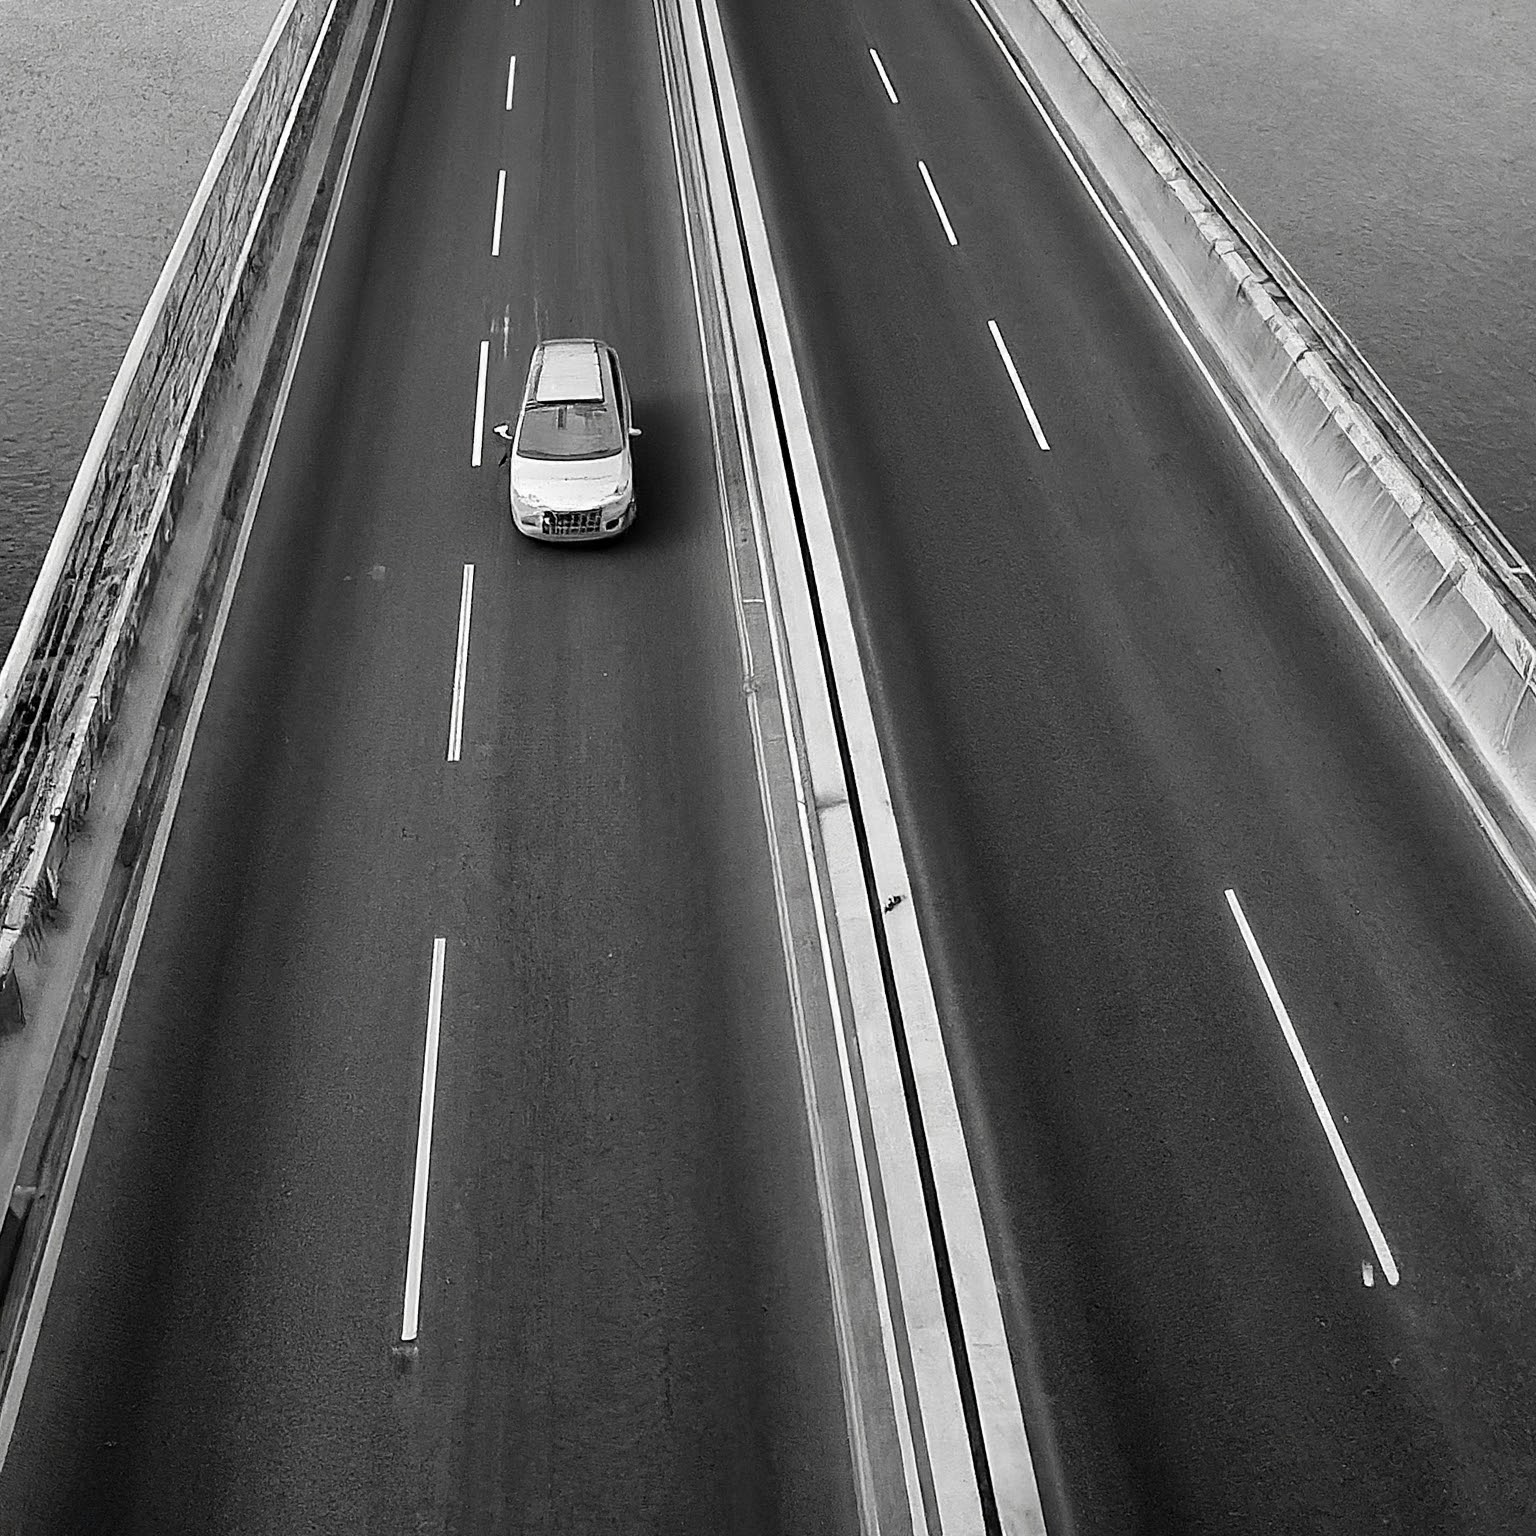
\includegraphics[width=0.3\textwidth]{textual/Figuras/image_fx_driving_a_car_across_a_bridge_black_and_white.jpg}
  \caption{Driving \emph{across} a bridge (Generated using ImageFX by Google).}
  \label{fig: across}
\end{figure}

From the primary idea of ``from one side to the other'', ACROSS can be broken down into four meanings:

%M: Só agora entendi que muitos erros de compilação estão acontecendo porque os exemplos do Linguex estão dentro de ambientes estruturados (itemize, enumerate etc.). Vai ser preciso tirar os exemplos de dentro desss ambientes. O exemplo é um ambiente em si mesmo.

\begin{description}
    \item [Movement over a Surface:] Similar to driving across the bridge, you can move across another surface such as a body of water (e.g.: a river, a lake) (Example~\ref{ex:10}).
\end{description}

    \ex. He sailed \emph{across} the lake.
    \label{ex:10}
    
\begin{description}
    \item [Perpendicular Position:] As described by~\textcite{bruckfield2011prepositions}, the bridge itself can also be described as located (static) across the river, such as in Example~\ref{ex:11}.
\end{description}

    \ex. The bridge \emph{across} the River Kwai has twelve arches. \label{ex:11}
    
\begin{description} 
    \item [Opposite Location:] The preposition ACROSS can also mean ``on the opposite side of'' something \parencite{cambridge-across}, like in Example~\ref{ex:12}.
\end{description}

    \ex. The library is just \emph{across} the road. 
    \label{ex:12}

\begin{description}
    \item [Distribution:] ACROSS can indicate something distributed throughout an area or something that spreads, occupies part of an area, or crosses some kind of surface \parencite{bruckfield2011prepositions}. See Examples~\ref{ex:13} and \ref{ex:14}.
\end{description}

    \ex. Voters \emph{across} the nation will elect a new president. \label{ex:13}

    \ex. The president was wearing the presidential sash \emph{across} his chest. \label{ex:14}


In the figurative sense, ACROSS can represent connections and how something permeates a wider area. For example, a smile spread \emph{across} a person's face can emphasize a broad and genuine sign of happiness. Similarly, in cloud computing, when you update files \emph{across} all your devices, the preposition highlights the interconnectedness between the network. The same way, in the business world, effective communication \emph{across} cultures is crucial for building strong international relationships; that is, \emph{across} underscores the need to bridge cultural gaps and establish connections among different groups.


\subsubsection{The Preposition THROUGH}

According to~\textcite{bruckfield2011prepositions}, THROUGH shares some similarities with ACROSS but extends to movement within a volume rather than over a surface. While ACROSS typically applies to two-dimensional spaces, the core meaning of THROUGH involves movement entering and exiting a three-dimensional space, such as:

\begin{description}
    \item[A Passage:] THROUGH is used to convey movement or direction from one side to the other within a passage or some kind of conduit (e.g., tunnels, channels, etc.), as illustrated in Example~\ref{ex:15}.
\end{description}

    \ex. He drove \emph{through} the tunnel. \label{ex:15}

    \begin{figure}[ht]
    \centering
    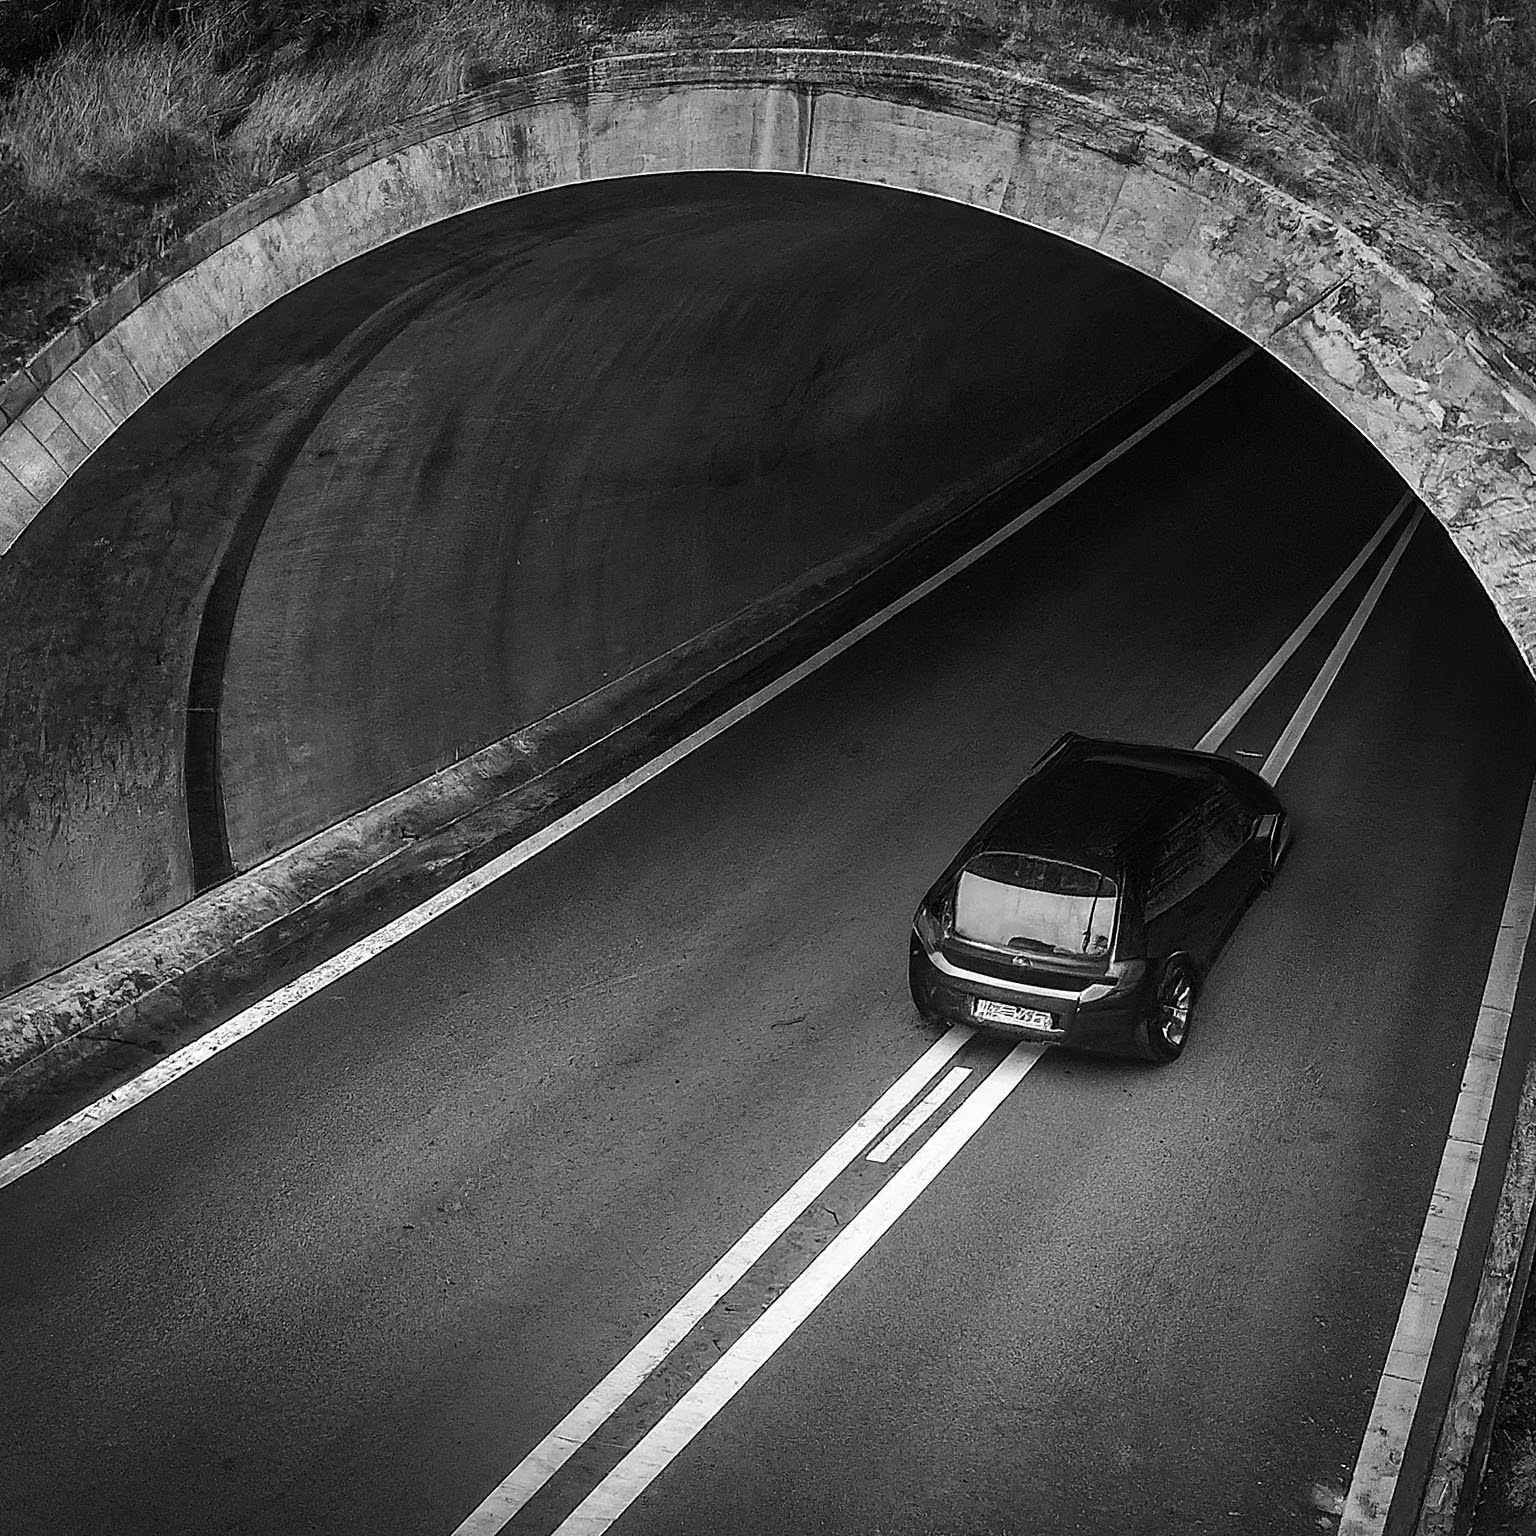
\includegraphics[width=0.3\textwidth]{textual/Figuras/image_fx_a_car_entering__a_tunnel_black_and_white_seen.jpg}
    \caption{Driving \emph{through} a tunnel (Generated using ImageFX by Google).}
    \label{fig:trough-ex-15}
    \end{figure}
    
\begin{description}
    \item[An Open Area:] THROUGH is also used to express movement from one side to the other within an open area, region, or place \parencite{cambridge-through}. See Example~\ref{ex:16}.
\end{description}

    \ex. To reach the museum, I had to walk \emph{through} the park. \label{ex:16}

\begin{description}
    \item[A Barrier:] THROUGH can signify movement past or penetrating a barrier or an obstacle, as illustrated in Examples~\ref{ex:17} and \ref{ex:18}.
\end{description}
    
    \ex. The car drove straight \emph{through} the gate. \label{ex:17}

    \ex. The man hammered a nail \emph{through} the board. (see Figure~\ref{fig:through}) \label{ex:18}
    
    \begin{figure}[ht]
    \centering
    
\includegraphics[width=0.3\textwidth]{textual/Figuras/image_fx_hammering_a_nail_through_a_wooden_board_black.jpg}
    \caption{Hammering a nail \emph{through} a wood board (Generated using ImageFX by Google).} \label{fig:through}
    \end{figure}
    
\begin{description}
    \item[Part of a Route:] THROUGH can also indicate a static location or movement along a route or path, as in Example~\ref{ex:19}.
\end{description}
     
    \ex. The sauna is \emph{through} the bathroom. \label{ex:19}


Beyond literal movement, the preposition THROUGH can be used figuratively. For instance, it can mean experiencing something indirectly, such as with a tool or medium (e.g., ``He was looking at the moon \emph{through} the binoculars''), describing a particular method (e.g., ``I like to build relationships \emph{through} trust and understanding'') or seeing from a perspective (e.g., ``I never saw their story \emph{through} their eyes'').


\subsubsection{The Preposition INTO}

The preposition INTO indicates ``movement in the direction of a container and the entry in the container'' \parencite{bruckfield2011prepositions}. It can be expanded into two specific meanings:

\begin{description}
    \item[Entering an Enclosure:] INTO is typically used for movement or direction ``to the inside or middle of a place, container, area, etc.'' (Example~\ref{ex:20}) \parencite{cambridge-into}.
\end{description}
    
    \ex. The boy kicked the ball \emph{into} the box. (see Figure~\ref{fig: into}) \label{ex:20}

    \begin{figure}[ht]
    \centering
    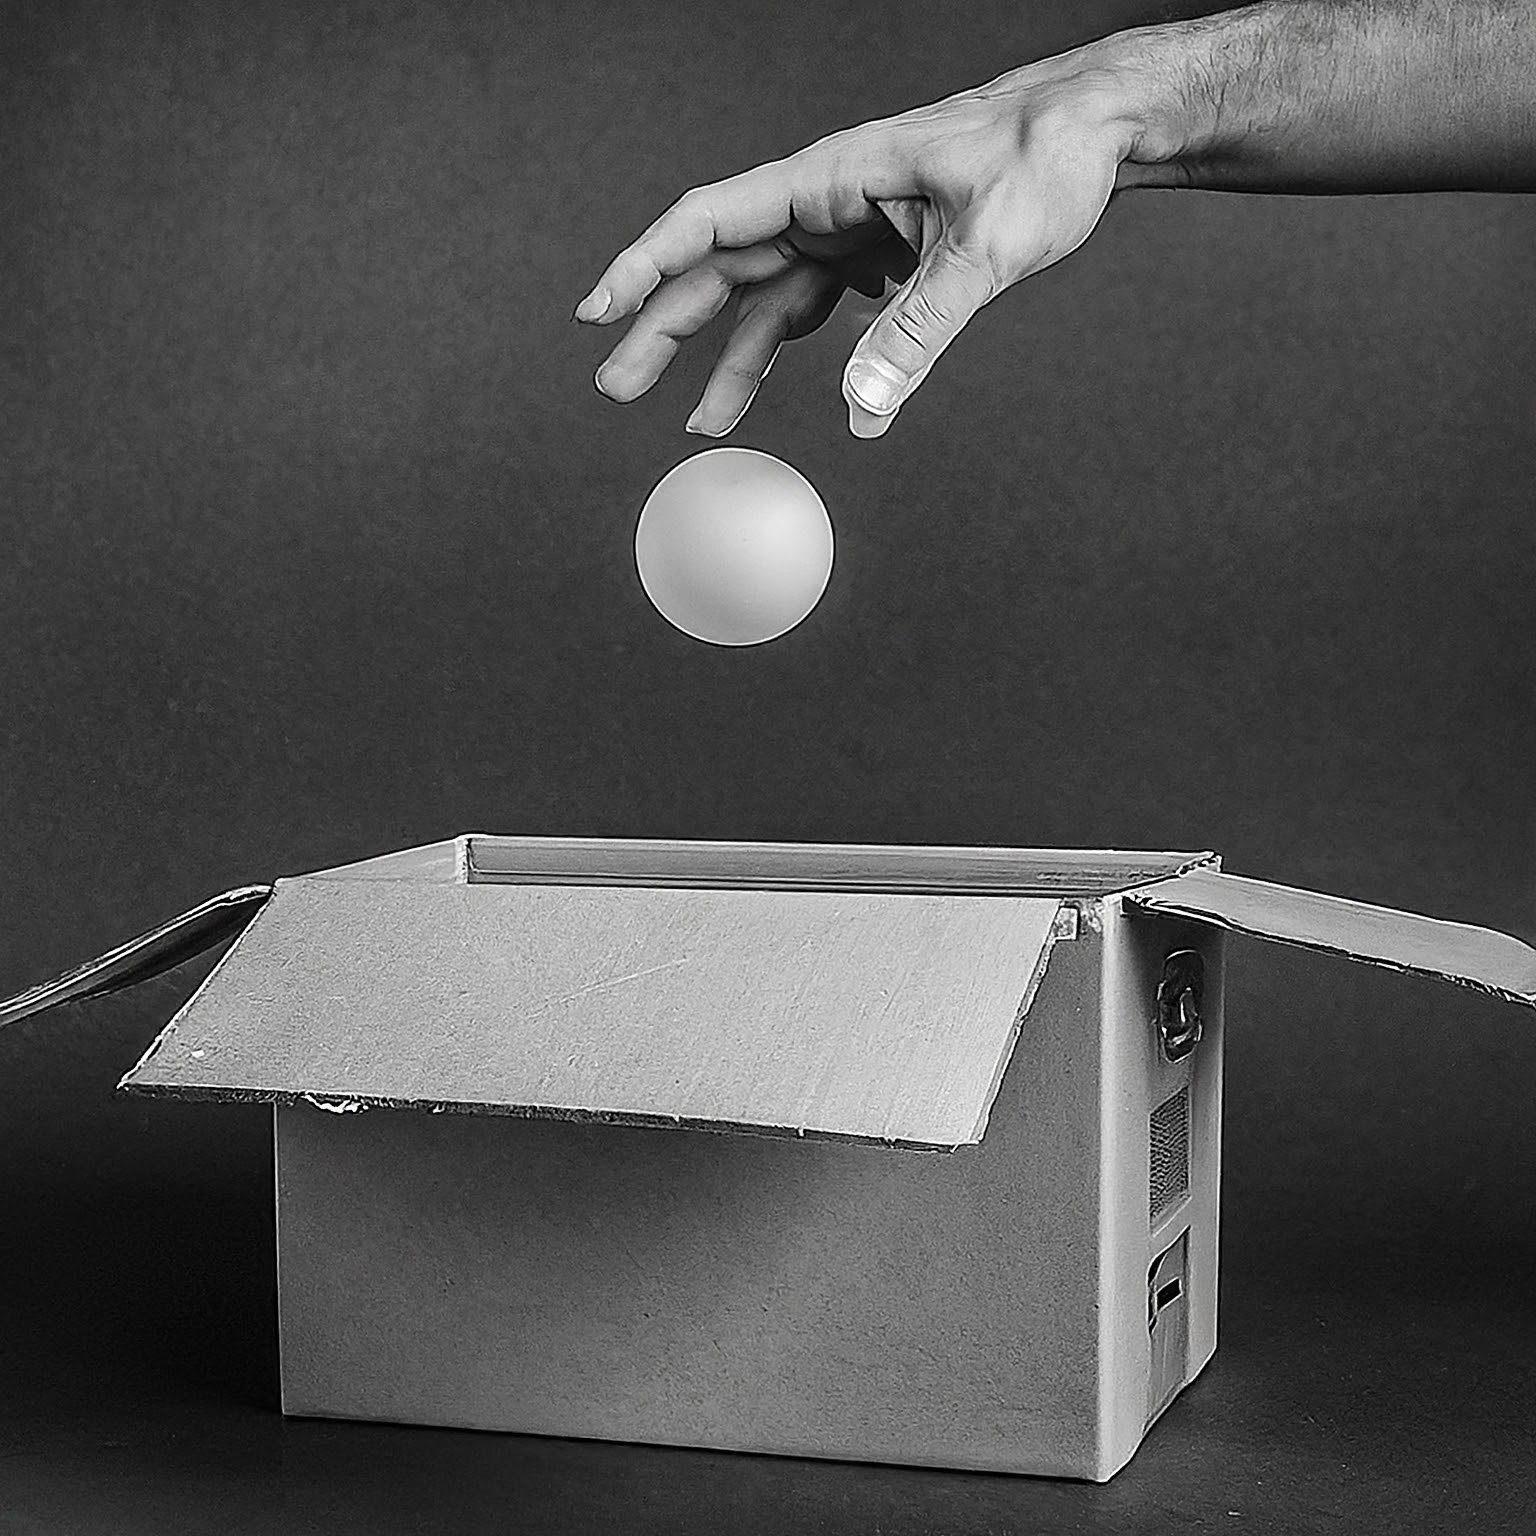
\includegraphics[width=0.3\textwidth]{textual/Figuras/image_fx_hand_throwing_a_ball_into_an_open_cardboard_b.jpg}
    \caption{The ball is going \emph{into} the box (Generated using ImageFX by Google).}
    \label{fig: into}
    \end{figure}
    
\begin{description}   
    \item [Movement with Force:] INTO indicates movement with force that usually results in collision with something else, but without moving inside of it, as in  Examples~\ref{ex:21} and \ref{ex:22}.
\end{description}
    
    \ex. The car crashed \emph{into} the wall. \label{ex:21}
    
    \ex. I wasn't looking where I was going and walked \emph{into} a lamppost. \label{ex:22}         


Beyond literal movement, INTO figuratively implies entering a new state (e.g.: ``She went \emph{into} a depression''), condition (e.g.: ``He went \emph{into} surgery''), transformation (e.g.: ``This software transforms your computer \emph{into} a piano''), etc. 


\subsubsection{The Preposition ONTO}
ONTO implies movement towards a surface, crossing a boundary into or onto the surface, regardless of its shape or position, as described by~\textcite{bruckfield2011prepositions} (see Figure~\ref{fig: onto}). 

    \begin{figure}[ht]
    \centering
    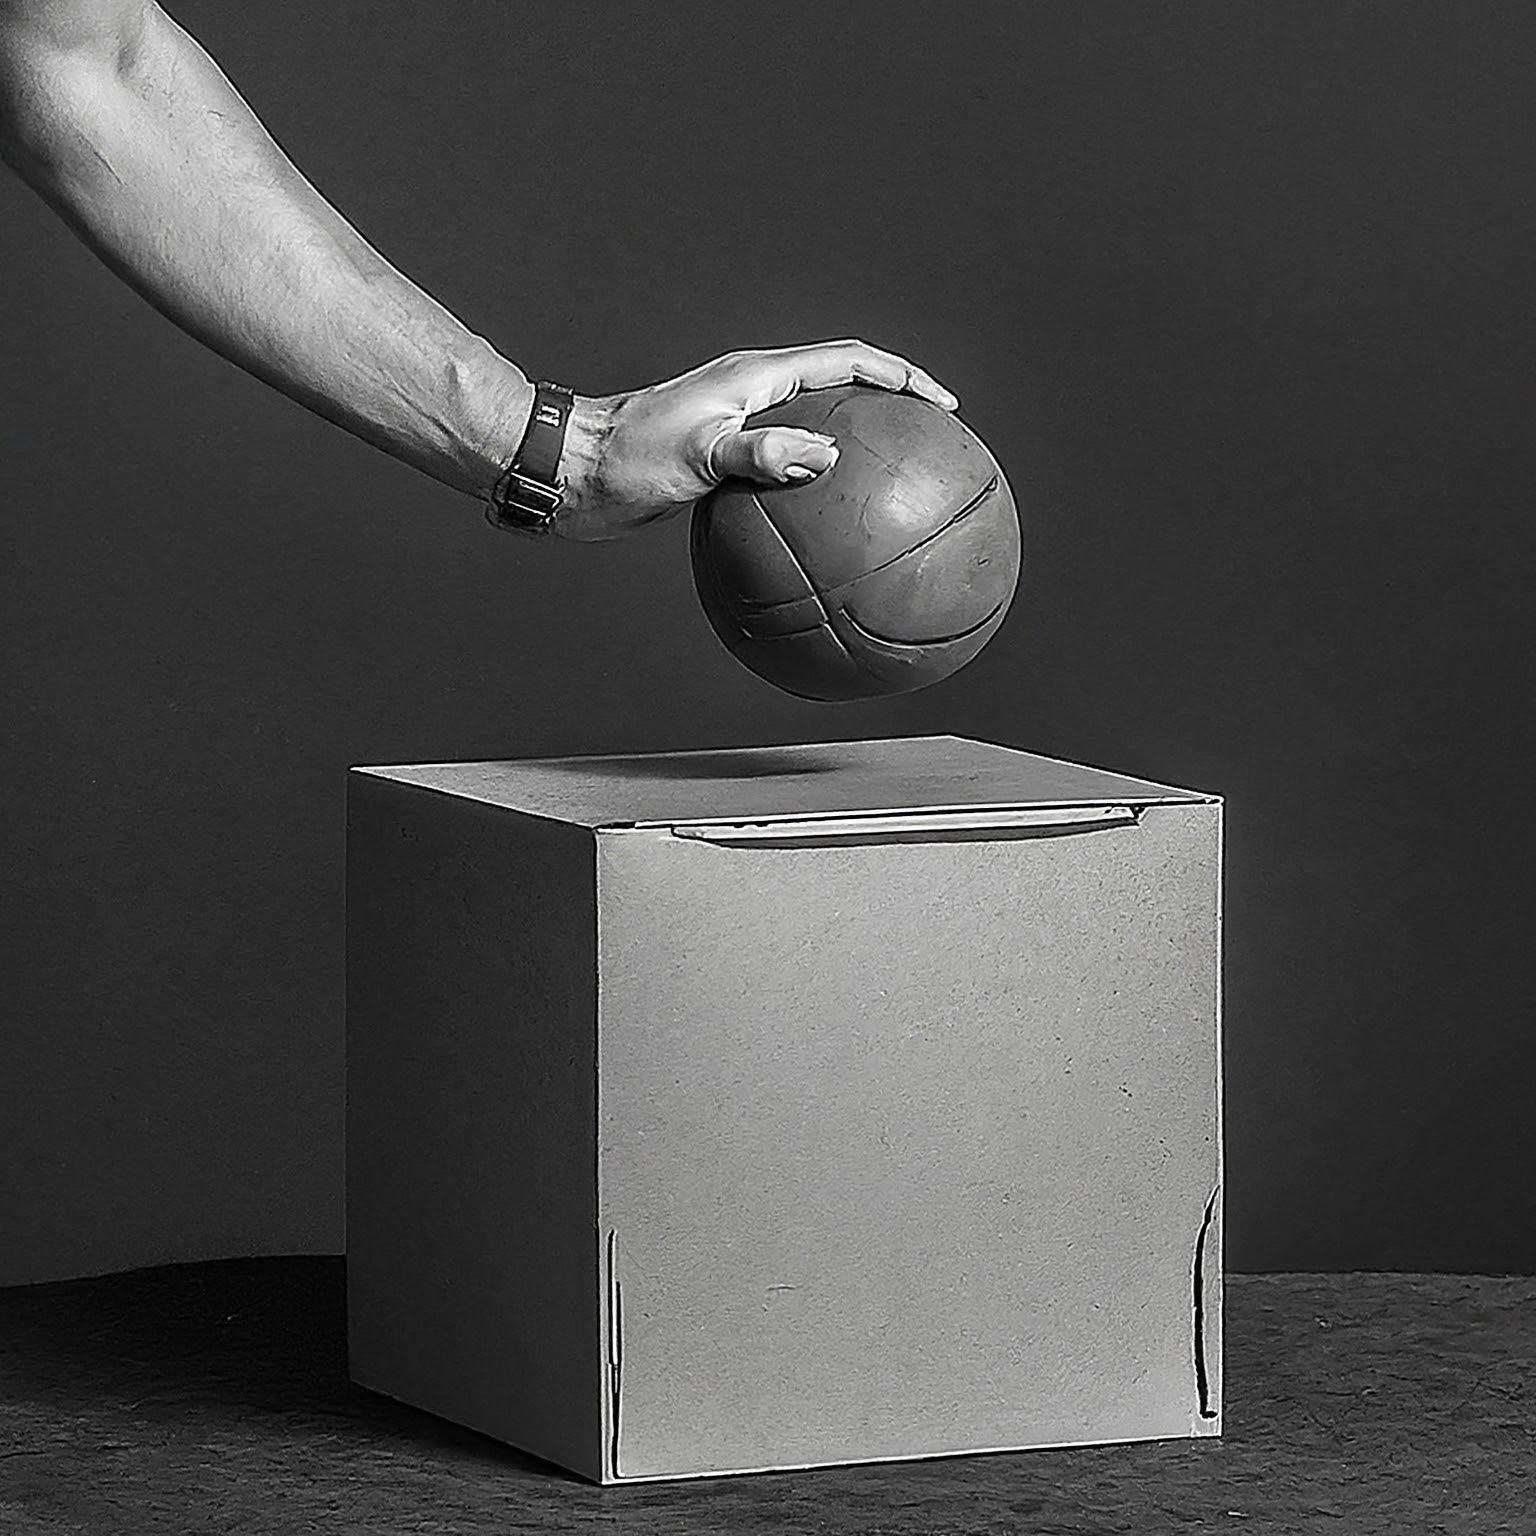
\includegraphics[width=0.3\textwidth]{textual/Figuras/image_fx_placing_a_ball_onto_a_closed_cardborad_box_bl.jpg}
    \caption{The ball is going \emph{onto} the box (Generated using ImageFX by Google).}
    \label{fig: onto}
    \end{figure}

\begin{description}
    \item[Movement towards a surface:] movement from an initial position to a final one on a surface (Example~\ref{ex:23}).
    
\end{description}
    
    \ex. I tossed the keys \emph{onto} the desk. \label{ex:23}
    
\begin{description}    
    \item [Sense of Attachment:] can imply a sense of attachment or pressure (Example~\ref{ex:24}).
\end{description}    
    
    \ex. He strapped the backpack \emph{onto} his shoulders and started hiking. \label{ex:24}
    

While both ONTO and ON relate to surfaces, \textcite{bruckfield2011prepositions} explains they differ based on movement versus final location. We use ONTO for movement towards a surface, whereas ON indicates something already resting on a surface. See Examples~\ref{ex: 25} and \ref{ex: 26}.

\ex. The father lifted the child \emph{onto} his shoulders. \label{ex: 25}

\ex. The father lifted the child \emph{on} his shoulders. \label{ex: 26}

In Example~\ref{ex: 25}, the child was initially in a lower position (e.g.: on the floor or on the baby pram) and was sat on the father's shoulders. In Example~\ref{ex: 26}, however, the father's shoulders was the initial support from which the child was lifted to a higher position.

Figuratively, ONTO goes beyond physical movement. For instance, it can suggest encountering something unexpectedly (``stumbling \emph{onto} a problem''), the final stages of a process (``putting the finishing touches \emph{onto} a plan''), awareness (``only one news channel was \emph{onto} the case''), or  attention (``the boss was \emph{onto} me) \parencite{cambridge-onto}. 


\subsection{Challenges in Translating Spatial Prepositions}
\label{subsec: Challenges in Spatial Prepositions}

This section explores the complexities of translating spatial prepositions between English (EN) and Brazilian Portuguese (PT-br), building upon the analysis of prepositional semantics. Particularly, it examines how PT-br often employs different prepositions, prepositional phrases, or parts of speech compared to EN to convey similar meanings.

\subsubsection{ACROSS \& THROUGH vs.\ `Através de': Similarities and Divergences}

In an preliminary study, \textcite{McCleary-Viotti-2004} provides valuable insights into the challenges of translating EN spatial prepositions like ACROSS and THROUGH using the PT prepositional phrase ``através de''. Their work draws on~\textcite{talmy2000towardb}'s proposition that languages select spatial elements from a finite universal inventory and combine them into ``schemas'' typically expressed by closed-class forms (such as prepositions). However, they argue that PT-br might rely more heavily on open-class forms (verbs and nouns) for spatial representation compared to EN. For instance, they present Example~\ref{ex:32}.

\ex. There is a barrier \emph{across} the road. (See Figure~\ref{fig:barrier}) \label{ex:32} \\
     ? Tem uma barreira \emph{através d}a estrada. \\
     Tem uma barreira (\emph{atravessada}) \emph{n}a estrada.

\begin{figure}[ht]
    \centering
    
\includegraphics[width=0.3\textwidth]{textual/Figuras/image_fx_a_barrier_across_the_road_black_and_white.jpg}
    \caption{A barrier \emph{across} the road (Generated using ImageFX by Google).}
    \label{fig:barrier}
\end{figure}
    
As discussed by~\textcite{McCleary-Viotti-2004}, while ``através de'' might seem like a direct translation of ACROSS, it aligns more closely with the schema of the preposition THROUGH, which, as discussed in Section~ \ref{sec: Spatial Prepositions}, represents movement in and out of a three-dimentional space, such as a volume. Nevertheless, in Example~\ref{ex:32}, ACROSS depicts ``the barrier'' as positioned parallel to ``the road'' (a two-dimensional space). To convey this concept, PT-br necessitates a verbal phrase, such as the past participle form ``atravessada'' (crossed), to emphasize the barrier's location in relation to the road's limits, highlighting the preference for open-class forms. To illustrate the similarity between ``através de'' and THROUGH, \textcite{McCleary-Viotti-2004} use Examples \ref{ex:33} and \ref{ex:34}. Note that, in this case, another prepositional phrase (por + a/o -- pelo, pela) is also possible.

\ex. Eles abriram um túnel \emph{através d}a/\emph{pel}a montanha. \label{ex:33}   \\
     They dug a tunnel \emph{through} the mountain.
      
\ex. A luz entrava \emph{através d}as/\emph{pel}as janelas do mosaico. (See Figure~\ref{fig:window})  \label{ex:34}  \\  
    The light entered \emph{through} the stained-glass windows. 

\begin{figure}[ht]
    \centering
    
\includegraphics[width=0.3\textwidth]{textual/Figuras/image_fx_light_shining_through_a_window_black_and_whit.jpg}
    \caption{Light shining \emph{through} a window (Generated using ImageFX by Google).}
    \label{fig:window}
\end{figure}


Examples~\ref{ex:33} and \ref{ex:34} illustrate motion within 3-D spaces (e.g.,``the montain'' and ``the window''), highlighting the parallels between the EN and PT-br prepositions in these contexts. However, this similarity should be approached with caution. As~\textcite{McCleary-Viotti-2004} point out, THROUGH and ``através de'' are not always interchangeable, as ``através de'' typically emphasizes the process of movement or action, rather than the final outcome. This distinction explains why the prepositional phrase in Examples~\ref{ex:35} and \ref{ex:36} is unacceptable in PT-br.

\ex. He hammered a nail \emph{through} the board. \label{ex:35}   \\
     ? Ele bateu/martelou um prego \emph{através d}a tábua. \\
     Ele bateu/martelou um prego \emph{que atravessou a}/\emph{n}a tábua.

\ex. Frankenstein's monster has a bolt \emph{through} his neck. \label{ex:36}   \\
     ? O monstro de Frankenstein tem um pino \emph{através d}o pescoço. \\
     O monstro de Frankenstein tem um pino (\emph{atravessado}) \emph{n}o pescoço.

In both Examples \ref{ex:35} and \ref{ex:36}, the scopes of ``através'' are final states (results) --- the nail gone through the board and the pin positioned in the creature's neck, respectively. This differs from ``através da montanha'' and ``através da janela,'' in that ``através'' emphasizes the process --- workers opening the tunnel and light entering the room. This distinction between describing a process (activity) versus a final state (result) is crucial for using the preposition effectively. In summary, as explained by~\textcite{McCleary-Viotti-2004}, ``através'' is only suitable when the phrase it precedes entails a process-type event structure (activity) or one that has as a sub-event a transition (achievement) or a process (accomplishment).


\subsubsection{The Versatility of PT-br Preposition `em'}

A descriptive study by~\textcite{oliveira2012cognitive} investigates the multiple meanings of the PT-br preposition ``em'' based on Langacker's Schematic Network model \parencite{langacker1987foundations}. The analysis of a massive dataset of journalistic texts (1.2 million words) published between 2007 and 2008 revealed that while ``em'' often conveys location, it can also take on other meanings unlike similar prepositions in other languages (e.g., French \emph{dans,} English \emph{in}). 
This versatility is further emphasized by the fact that it frequently appears blended with articles, numerals, and demonstrative pronouns through the root ``n-''. Due to its broader range of usage, ``em'' is highly dependent on the surrounding text for its specific meaning.

One way to understand the complexities of ``em'' is by examining the schemas associated with it. The two most  prototypical meanings, as explained by~\textcite{oliveira2012cognitive}, are the CONTAINER (see Figure~\ref{fig: container}) and CONTACT (see Figure~\ref{fig: contact}). The CONTAINER schema captures the notions of `inclusion' and `closure,' as illustrated in Example~\ref{ex:container}. The CONTACT schema, on the other hand, focuses on the concept of `support,' where ``em'' describes the relationship between the Figure and a surface it interacts with (Ground) (see Example~\ref{ex:contact}).

\ex. Imaginem o suco \emph{num} copo. \newline \label{ex:container}
[Imagine the juice \emph{in} a glass.]

\begin{figure}[ht]
\centering
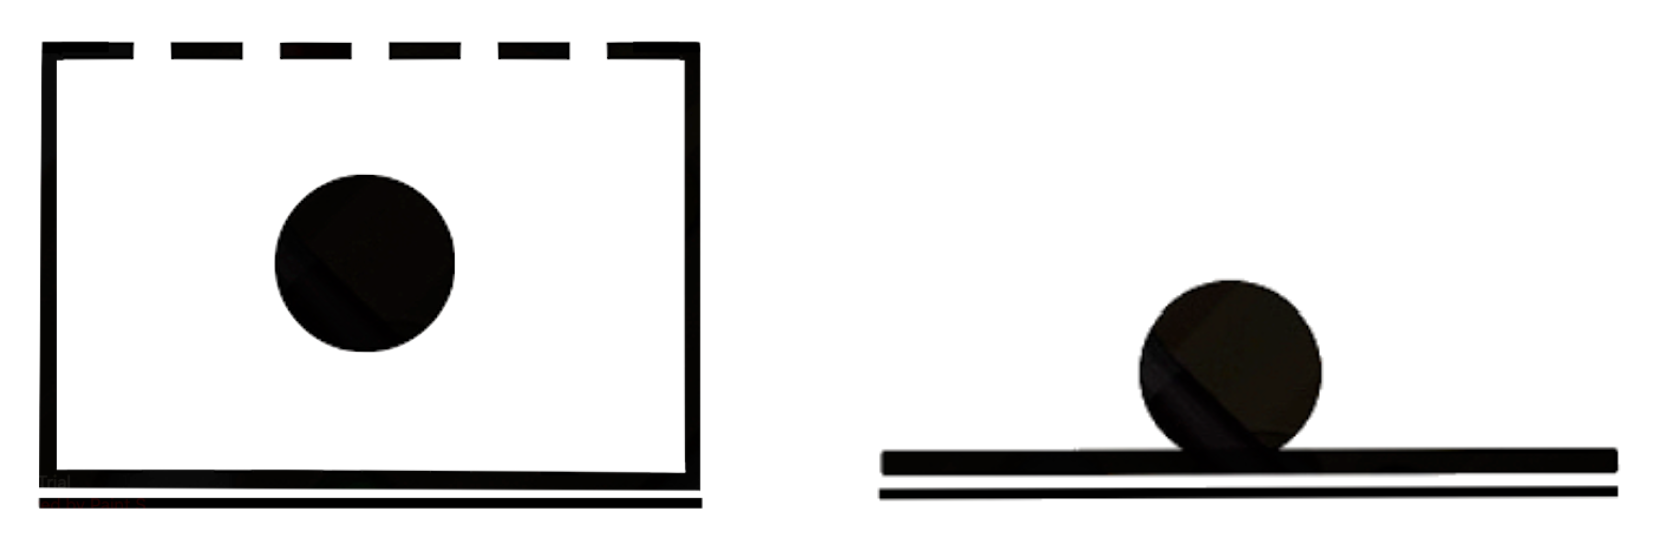
\includegraphics[width=0.6\textwidth]{textual/Figuras/Untitled design.png}
\caption{The CONTAINER vs. CONTACT schemas.}
\label{fig: container}
\end{figure}

\ex. Se for preciso, vamos acampar \emph{na} quadra. (E. de Minas -- Aug.05.2008) \newline [If necessary, we shall camp \emph{on} the court.] \label{ex:contact}

\begin{figure}[ht]
\centering

\includegraphics[width=0.6\textwidth]{textual/Figuras/Untitled design-2.png}
\caption{Conceptualizations: ``\emph{num} copo'' vs. ``\emph{na} quadra'' (Generated using ImageFX by Google).}
\label{fig: contact}
\end{figure}


However, the concept of movement with ``em'' presents an interesting nuance within the schema framework. Although typically signifying location rather than movement, as \textcite{oliveira2012cognitive} suggests, in dynamic contexts, ``em'' can locate an object at the endpoint of a Path, implying a ``caused motion'' schema. As illustrated in sentences \ref{ex:em-into} and \ref{ex:em-at} from \textcite{oliveira2012cognitive},  where ``em'' highlights the final location of the sewage and thrown objects, irrespective of the surface being a pond, field, or something else entirely. This suggests that schemas associated with ``em'' might be more flexible than initially conceived,  potentially incorporating a ``caused motion'' aspect in specific contexts where movement is implied by the situation (e.g., throwing, dumping).

\ex. Depoimentos de moradores, fotografias, vídeos e a análise da água mostram que esgoto sem tratamento está sendo despejado \emph{na} lagoa. (Estado de Minas – Aug.06.2008) \label{ex:em-into} \newline
[Residents’ reports, photos, videos, and the analysis of the water show that untreated sewage has been dumped \emph{into} the pond.]

\ex. Além de uma faixa com os dizeres “Queremos um time de verdade”, bonecas, pipocas e bananas foram jogadas \emph{no} gramado. (Estadão -- Jun.24.2008) \label{ex:em-at} \newline
[Besides a banner which read “We want a real team”, puppets, popcorn and bananas were thrown \emph{onto} the field.]


In addition, \textcite{Ferreira-Basso-2020} clarify that the directional or goal-related interpretation of ``em'' is a false syncretism arising from the presence of verbs indicating movement in the structure. In sentences like Example~\ref{ex:em-goal}, ``em'' emphasizes that the Figure (the entity) ends up \emph{inside} the Goal after the movement, establishing a static locative relationship at the event's conclusion. However, in structures without such verbs, like in Example~\ref{ex:em-loc}, ``em'' is interpreted as merely locative, describing the Figure's static position relative to the Ground (the reference point), thereby reinforcing its understanding as a locative preposition.

\ex. Pedro correu \emph{na} farmácia.\label{ex:em-goal} \newline
[Peter ran \emph{to} the pharmacy.]

\ex. Ana almoçou \emph{no} shopping.\label{ex:em-loc} \newline
[Ana had lunch \emph{at} the shopping mall.]


\textcite{oliveira2012cognitive} also explores situations where the Figure lacks a physical presence. In these cases, the Ground, also referred to as the ``Medium'', can involve the absence of something within it, like a ``hole'' in a wall. These missing parts are called ``empty spatial trajectors.'' According to~\textcite{oliveira2012cognitive}, the viewer mentally completes the missing part of the surface, creating a space for the ``hole''. In this configuration, the boundary of the Ground and the external boundary of the Figure overlap. Example~\ref{ex: em-into-through} illustrates this case where ``em'' could be translated as either INTO or THROUGH in EN, depending on more specific details of the Path taken by the drill. In PT-br, if we want to emphasize the crossing aspect, we can use ``atravessado'' for THROUGH. Figure~\ref{fig: hole-wall} demonstrates the concept in PT-br, where the broken line depicts the completed wall and the shaded region represents the hole. Additionally, Figure~\ref{fig:hole-wall2} shows the different scenarios for ``em'' as INTO vs. THROUGH.

\ex. O homem furou um buraco \emph{na} parede. \label{ex: em-into-through} \newline
[The man drilled a hole \emph{into}/\emph{through} the wall.] 


\begin{figure}[ht]
\centering
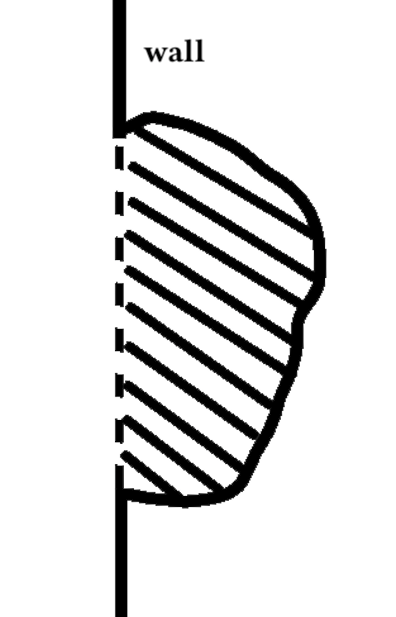
\includegraphics[width=0.2\textwidth]{textual/Figuras/Screen Shot 2024-05-28 at 19.46.20.png}
\caption{Closure of the landmark during conceptualization in PT-br.}
\label{fig: hole-wall} 
\end{figure}

\begin{figure}[ht]
\centering

\includegraphics[width=0.6\textwidth]{textual/Figuras/Untitled design-4.png}
\caption{INTO (left) vs. THROUGH (right): ``um buraco  \emph{na} parede'' (Generated using ImageFX by Google).}
\label{fig:hole-wall2} 
\end{figure}

As emphasized by~\textcite{oliveira2012cognitive}, entities like holes, cracks, perforations of any sort must be construed the same way as any concrete object. Besides, the idea of inclusion might not be so emphasized using ``em'' in PT-br as in EN with INTO, for instance. The complex  ``dentro de'' (inside; in) is the one to convey ``inclusion'' in PT-br.

\vspace{0.5em} % Adjust the value (e.g., 1em) to increase or decrease the gap

To sum up, in Section~\ref{sec: translating-spatial}, we detailed the challenges of translating spatial prepositions between EN and PT-br, particularly focusing on issues like polysemy, where a single EN preposition may correspond to multiple meanings, complicating its translation into PT-br. Additionally, the structural differences between the two languages mean that EN often relies on prepositions to convey spatial relationships, while PT-br typically expresses these meanings through verbs. As we transition to the next topic, it is critical to examine these complexities to fully understand the translation difficulties at stake.


\section{Neural Machine Translation}
\label{sec: nmt}

\epigraph{Going to Mars is less relevant than being understood. Language is the tool to solve all the other problems. \\ \hfill --- Marco Trombetti, Co-Founder \& CEO, Translated, Pi Campus}

This section explores the evolution of MT, from early approaches to the state-of-the-art: Neural Machine Translation (NMT). We delve into NMT's architecture, including its encoder-decoder structure and attention mechanism, while also discussing its limitations. We then compare recurrent and transformer-based NMT systems, contrasting their information flow handling. Finally, we discuss the emerging impact of Large Language Models (LLMs) on NMT and the challenges associated with their integration.


\subsection{A Response to Translation Challenges}

The dream of automatic language translation has captivated researchers since the dawn of computing. Early efforts, like those undertaken during World War II code-breaking, laid the groundwork for the field. For many years, Statistical Machine Translation (SMT) and Rule-Based Machine Translation (RBMT) dominated the MT landscape, each offering valuable contributions. However, both approaches encountered limitations \parencite{koehn2020neural}.

Alternatively, according to~\textcite{koehn2020neural}, NMT has emerged as a  significant advancement in recent years in an attempt to overcome the issues presented by previous methods. For instance, as~\textcite{koehn2012statistical} points out, SMT systems often struggled with rare or unseen words, lack of context awareness, and limited ability to capture complex relationships within a sentence. RBMT, on the other hand, faced challenges in creating comprehensive and accurate linguistic rules, handling idiomatic expressions and language nuances, and adapting to new languages or domains \parencite{shiwen2014rule}.

This shift from word-for-word translation to an approach that considers context and provides better resuts on long-range dependencies allows NMT to generate more natural and accurate translations. According to~\textcite{lakew2019multilingual}, state-of-the-art NMT systems achieve this by relying on a key triad: an \emph{encoder} that analyzes the source sentence, a \emph{decoder} that generates the target language translation, and an \emph{attention} mechanism that allows the decoder to focus on relevant parts of the source sentence during translation (see Figure~\ref{fig: Encoder-decoder-attention} for a visual representation). However, these systems differ in how they handle the source sentence, leading to variations in performance.

\begin{figure}[ht]
\centering
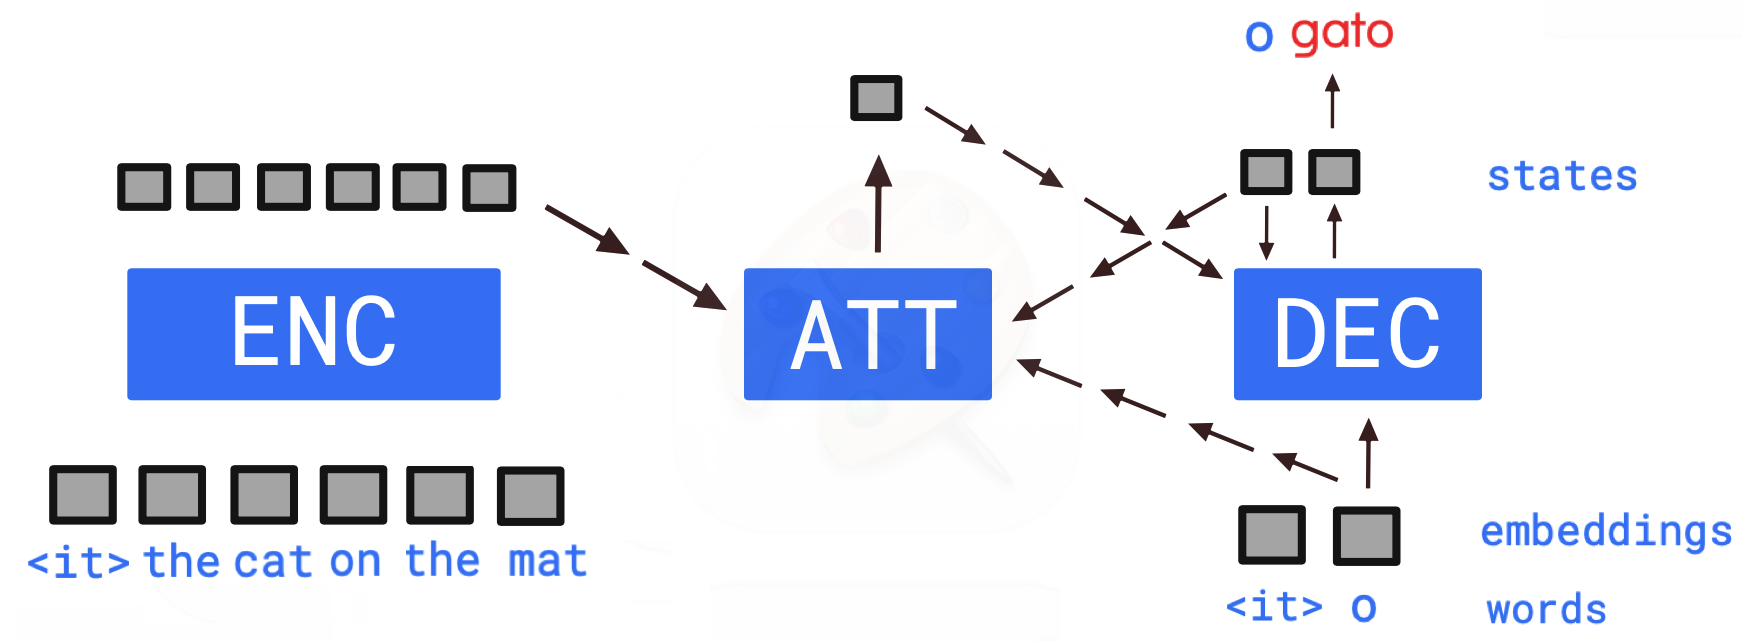
\includegraphics[width=0.8\textwidth]{textual/Figuras/enc-dec.png}
\caption{The encoder-decoder-attention NMT architecture, based on an illustration by~\textcite{lakew2019multilingual}. The \emph{encoder} reads the input sentence (``the cat on the mat'') word by word. For each word, it creates a state capturing its meaning. The \emph{decoder} then builds the translated sentence (``o gato'') one word at a time. To do this, it considers the previous word (``o''), its own internal state, and a special \emph{attention} mechanism. Attention allows the decoder to focus on relevant parts of the encoder's states (e.g., ``cat'') to generate the correct translation (``gato'').}
\label{fig: Encoder-decoder-attention} 
\end{figure}

As \textcite{lakew2019multilingual} explains, the core of NMT lies in how the encoder and decoder work together. The encoder acts like a translator, mapping the source sentence into a sequence of state vectors that capture each word's meaning and its connection to others. The decoder then builds the target language word by word, relying on three key elements: its internal memory of previously translated words, the last generated word for fluency, and the ingenious attention mechanism \parencite{luong2015effective}. This mechanism acts like a filter, highlighting the most relevant parts of the encoded source sentence for each target word, allowing the decoder to translate complex sentences.

Pioneering NMT approaches (like those by \textcite{sutskever2014sequence}) rely on recurrent neural networks (RNNs) to analyze the source sentence word by word. Stacking multiple RNN layers creates ``deep'' recurrent NMT, enabling them to capture some context within the sentence. However, these models still struggle with long-range dependencies, meaning they can have difficulty understanding how words far apart in the sentence relate to each other, particularly in complex sentences. Despite their theoretical flexibility, RNN-based NMT can be challenging and slow to train \parencite{lakew2019multilingual}.

Transformer-based NMT systems, introduced by~\textcite{Vaswani-2017}, takes a fundamentally different approach. They leverage a transformer architecture that analyzes the entire source sentence at once using an attention mechanism. This is in contrast to recurrent NMT, which processes information sequentially. By analyzing the entire sentence at once, transformers can effectively capture long-range dependencies between words, leading to generally more parallelization and better translation quality compared to recurrent NMT.

\begin{figure}[ht]
\centering
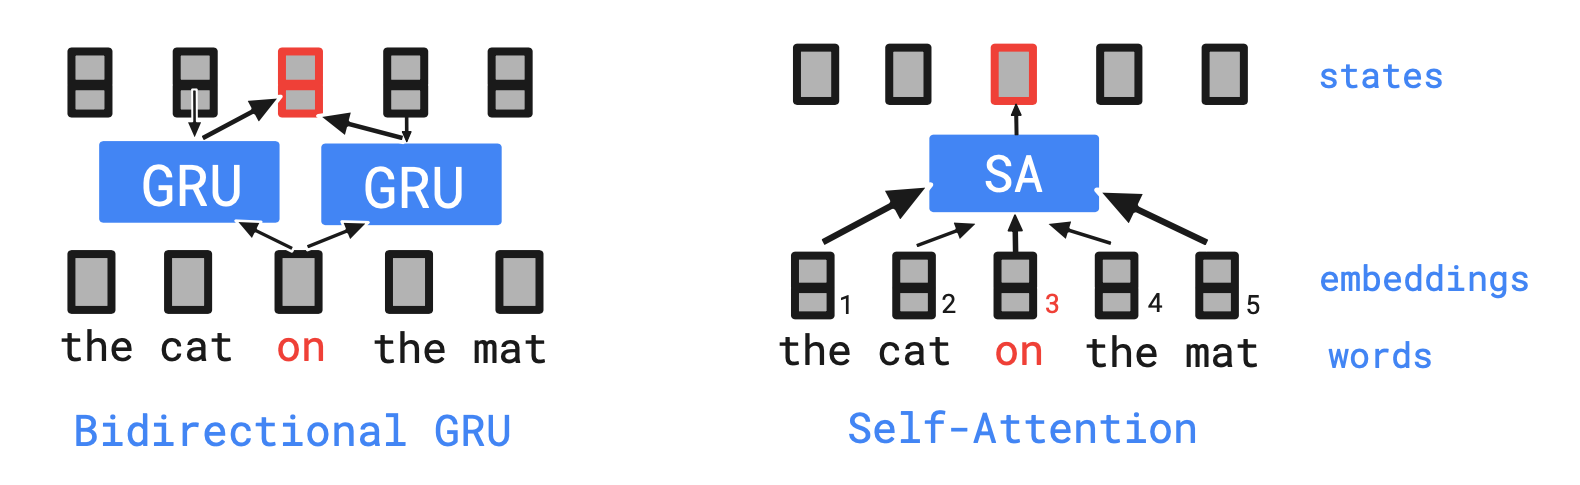
\includegraphics[width=0.9\textwidth]{textual/Figuras/self.png}
\caption{How Encoders Read Sentences: Recurrent vs. Transformers (based on \textcite{lakew2019multilingual}).}
\label{fig: rnn-transformers} 
\end{figure}

Figure~\ref{fig: rnn-transformers} depicts the differing approaches of RNNs, such as LSTMs, and transformers within NMT encoders when handling sentences. RNNs (on the left) process words sequentially, like building blocks (e.g., ``the'' then ``cat''). Here, two processing units (``GRU'') create the state for ``on''. In contrast, transformers (on the right) analyze all words at once (``the'', ``cat'', ``on''). They use a self-attention mechanism (marked by SA) to understand word order and create the state for ``on''. This parallel processing allows transformers to work more efficently than RNNs, leading to better results in NMT.

In essence, the potency of the transformer, as detailed in~\textcite{lakew2019multilingual}, stems from its architecture built upon a series of ``encoder-decoder layers'' operating in an autoregressive manner. This means it relies on the previously generated element to predict the next one, analyzing information step-by-step. Notably, both the encoder and decoder can consist of identical layers, each containing two sub-layers: a multi-head ``self-attention'' mechanism and a position-wise ``feed-forward'' network. The first highlights the most important connections between words within the sentence, while the second adds extra processing power for deeper analysis. However, the decoder incorporates an additional multi-head attention layer that allows it to focus on the outputs generated by the encoder. This multi-head attention mechanism effectively enables the use of multiple attention functions while maintaining similar computational costs to a single attention function, ensuring coherent and accurate translation.


\subsection{A Promising Approach with Emerging Limitations}

A decade after publishing his seminal work on ``Statistical Machine Translation,'' \textcite{koehn2020neural} revisits the field in ``Neural Machine Translation,'' highlighting a dramatic shift in translation technology. Deep learning architectures, particularly neural networks, have become the dominant paradigm. As the author points out, this shift has brought impressive improvements in translation quality, but also introduced new challenges.

One major hurdle for NMT is \textit{domain mismatch}. As highlighted by~\textcite{koehn-knowles-2017-six}, NMT systems often struggle when translating text from specific domains that differs significantly from the data they were trained on. This is because these specialized domains have unique vocabulary and phrasings that may be uncommon in general training data. In such cases, NMT models can prioritize accuracy over idiomacity, resulting in translations that sound grammatically correct but miss the intended meaning. 

An interesting approach to address this challenge involves domain adaptation. Here, a customized version of the model is further refined by training it on additional data from the target domain for a shorter period. This two-step process, championed by~\textcite{LuongPM15, FreitagA16}, leverages the strengths of both general and domain-specific training data. This can lead to more accurate use of terminology in NMT, particularly for specialized domains like legal documents or medical reports \parencite{matusov-etal-2019-customizing, mirkin2015personalized}.

Furthermore, NMT exhibits a ``steeper learning curve'' compared to SMT when it comes to the \textit{amount of training data} required. In simpler terms, NMT models need significantly more data exposure to achieve good performance. Consequently, NMT excels in high-resource settings (abundant training data) but struggles with limited data, resulting in lower quality outputs (as observed by~\textcite{koehn-knowles-2017-six}). This vulnerability to data scarcity can lead to another issue -- \emph{overfitting}. Imagine a student who memorized every answer in a textbook failing to answer slightly rephrased questions. Similarly, NMT models trained on a limited dataset might do well at translating those specific sentences but struggle with entirely new vocabulary or sentence structures.

Another thing is that, while NMT excels at handling extremely \textit{low-frequency words} (e.g., proper nouns) thanks to sub-word level operations (like byte-pair encoding), a key challenge remains: translating rare words belonging to highly inflected categories (e.g., verbs). Previously, according to~\textcite{koehn-knowles-2017-six}, research suggested that NMT usually struggles with rare words in general \parencite{LuongPM15, sennrich-etal-2016-neural} due to their smaller vocabularies. However, their study comparing NMT and SMT systems of similar quality for German-English translation found that NMT actually outperforms SMT on very infrequent words.

\textit{Very long sentences} pose a particular challenge for NMT, with quality dropping significantly compared to shorter ones. This was especially true for early models \parencite{cho2014properties, pouget2014overcoming}. Interestingly, recent research suggests that a simpler factor, the mismatch between training and testing data lengths, could also contribute to this performance drop \parencite{varis-bojar-2021}. To investigate this challenge and the potential limitations of the attention mechanism, \textcite{koehn-knowles-2017-six} employed a powerful English-Spanish NMT system to translate news articles from a standard dataset. They categorized the translations by their original length in the source language and evaluated the quality for each group. While NMT generally outperformed SMT, a surprising finding emerged: for very long sentences (over 80 words), the NMT system produced significantly shorter translations, often omitting details. This suggests that the attention mechanism might struggle with capturing the full context in extremely long sentences.

According to~\textcite{koehn-knowles-2017-six}, although common in NMT, attention mechanisms may not directly map to traditional \textit{word alignment} models. Originally, the intention behind incorporating attention in NMT was to establish word alignments. This involved creating a probability distribution that assigned weights to source words based on their relevance to each target word, treating the source sentence more like a bag-of-words. Despite this initial goal, there is an argument to be made that attention in NMT does not fulfill the same role as word alignment in SMT. Unlike SMT's direct word-to-word correspondence between source and target languages, NMT's attention focuses on highlighting relevant source words for target word generation.

Lastly, \textit{beam search}, a technique for finding the best translation in both SMT and NMT, seems to have a sweet spot. While increasing the number of explored possibilities (beam size) generally improves translation quality, \textcite{koehn-knowles-2017-six} have observed a ``beam search curse''. Beyond an optimal beam size (usually around 30-50), translation quality actually worsens. This seems to be because wider beams favor shorter translations, leading to a drop in quality despite exploring more options. Techniques like score normalization by translation length can help mitigate this issue, but there is a clear limit to how much beam size can be increased for optimal NMT performance.

Overall, NMT offers a valuable tool for communication despite limitations like domain mismatch, data scarcity, and challenges with long sentences. These limitations contribute to the current focus of NMT, as argued by~\textcite[19]{koehn2020neural}, which is ``not to achieve perfect translation but to drive down error rates of machine translation systems''. This means that, while current NMT systems may not achieve perfect translations and can struggle with deeper meaning, they often generate understandable text for most audiences -- including casual users, students, and professionals -- who can handle some ambiguity.


\subsection{The Rise of Large Language Models}

LLMs, powered by the transformer architecture, have made significant strides in the field of NLP \parencite{zhao2023survey}. These complex and robust AI systems, trained on extensive datasets of text and equipped with billions of parameters, exhibit a notable ability to comprehend and respond to human language.

Models such as ChatGPT have demonstrated their capabilities in a variety of tasks. They are able to engage in conversations, understand user intent, and provide informative or helpful responses. This is due to their ability to analyze large amounts of textual data and identify patterns that resemble human conversation \parencite{yuhan-etal-2023-unleashing}. Consequently, LLMs can adjust their communication style to match the user and generate responses that are contextually relevant. This progression is similar to the transition from statistical methods to neural networks in MT, with pre-trained models paving the way for the development of more advanced LLMs over the past few years. This trend is illustrated in Figure~\ref{fig: LLM-releases}, which shows the increasing number of LLMs released.

LLMs can be generally categorized into two main types, each with a distinct approach based on its underlying architecture \parencite{yuhan-etal-2023-unleashing} (as outlined in Table~\ref{tab:pre-trained-models}). \emph{Encoder-Decoder} models, recognized for their versatility, combine an encoder that interprets the input with a decoder that generates an output based on the encoded information. This dual functionality enables them to perform well in tasks such as translation or sentence completion. On the other hand, \emph{Decoder} models specialize in generating outputs. They employ a decoder to produce text or other formats based on specific conditions or context, similar to generating text in response to prompts.

\begin{table}[htb]
\footnotesize
\centering
\begin{tabular}{lccl}
\toprule
\textbf{Model} & \textbf{Publishing Agency} & \textbf{\#Parameters} & \textbf{Architecture} \\ \midrule
T5 \parencite{JMLR:v21:20-074} & Google Brain  & 220M--11B & Encoder-Decoder \\
ERNIE-3.0 \parencite{sun-at-al-2021}  & Baidu & 10B & Encoder-Decoder \\
ERNIE-3.0 Titan \parencite{wang-at-al-2021}   & Baidu  & 260B & Encoder-Decoder \\
PaLM-2 \parencite{google_palm2_2023}  & Google & 1.04B--2.7B & Encoder-Decoder \\
GLM-130B \parencite{zeng2023glm130b}  & Zhipu.AI  & 100M-515M & Encoder-Decoder \\ 
\midrule
GPT-2 \parencite{brown-at-al-2020}  & OpenAI  & 1.5B & Decoder \\
GPT-3 \parencite{ye2023comprehensive} & OpenAI  & 2.6B--200B & Decoder \\
GPT-3.5 \parencite{lin2023comparison}  & OpenAI  & - & Decoder \\
\midrule
FLAN \parencite{wei2022finetuned}  & Google & 137B & Decoder \\
InstructGPT \parencite{ouyang2022training}  & OpenAI & 1.3B--175B & Decoder \\
PaLM \parencite{chowdhery2022palm}  & Google & 8B-540B & Decoder \\
OPT \parencite{zhang2022opt}  & Meta AI  & 6.7B--175B & Decoder \\
Bloom \parencite{workshop2023bloom}  & HuggingFace  & 560M-176B & Decoder \\
FLAN-PaLM \parencite{chung2022scaling}  & THUNLP  & 250M--11B & Decoder \\
LLaMA \parencite{touvron2023llama}  & Stanford  & 780M-65B & Decoder \\
\bottomrule
\end{tabular}
\caption{Overview of Large Pre-training Models \parencite{yuhan-etal-2023-unleashing}.}
\label{tab:pre-trained-models}
\end{table}

The conventional methods of developing dedicated systems for specific NLP tasks can be both time-consuming and resource-intensive. This has led to a new direction in research: prompt engineering \parencite{qiao-etal-2023, zhou-etal-2022-prompt}. This novel approach enables the rapid adaptation of LLMs to specific tasks, providing a more efficient and flexible alternative. Research suggests that prompting LLMs can achieve performance results that are on par with, or even exceed, those of specialized systems across various NLP tasks, including sentiment analysis and question answering \parencite{Radford2019LanguageMA}.

\begin{figure}[htb]
\centering
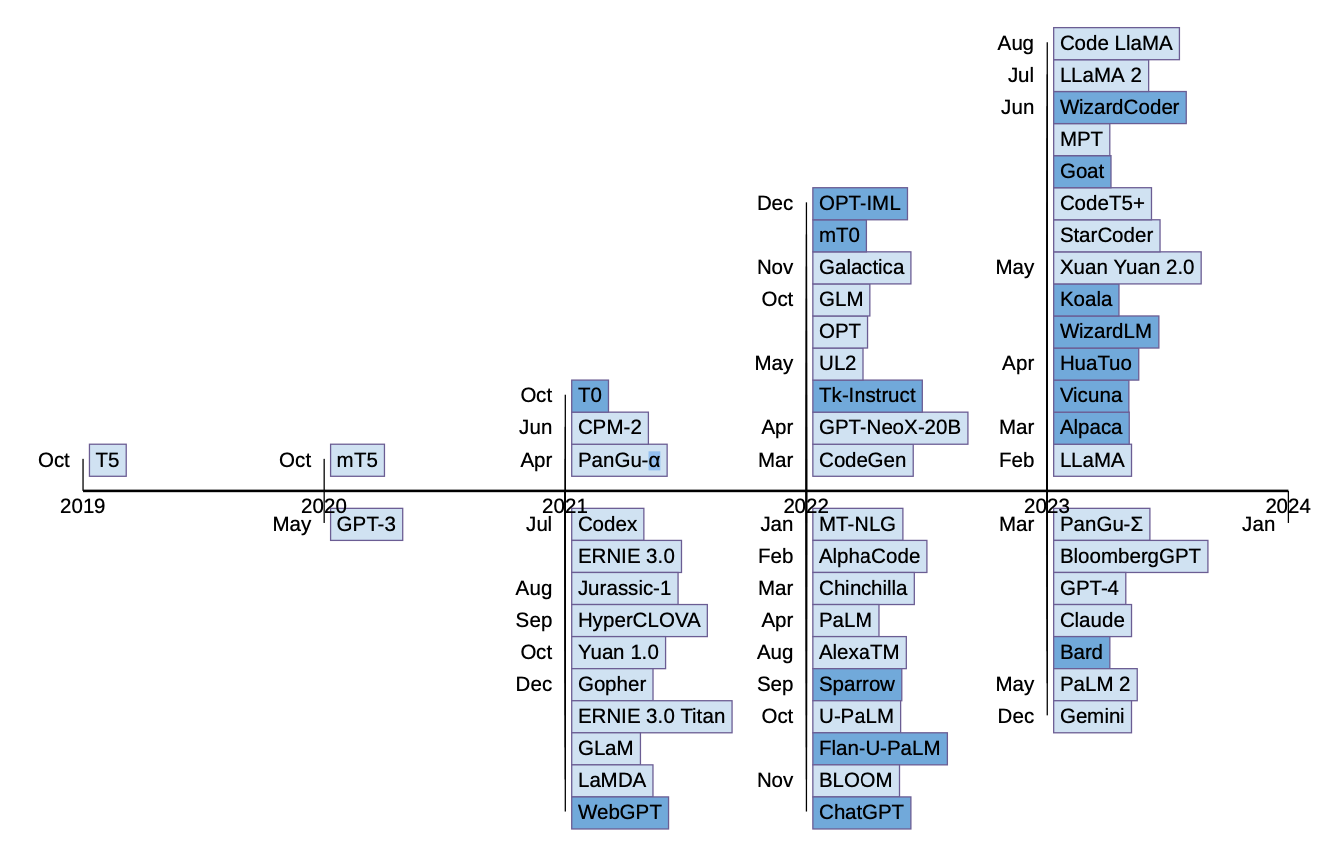
\includegraphics[width=1\textwidth]{textual/Figuras/LLM-releases.png}
\caption{Chronological LLM Release Trends, as illustrated by~\textcite{naveed2024comprehensive}. This chart shows a rise in open-source, instruction-tuned models (dark blue, top) compared to pre-trained models (light blue) and close-source (bottom). It highlights the evolving landscape of NLP.}
\label{fig: LLM-releases} 
\end{figure}

The adaptability of LLMs through prompts has significant implications for MT. \textcite{yuhan-etal-2023-unleashing} demonstrate that LLMs can achieve remarkable translation outcomes with just a few-shot translation examples, despite being trained primarily on multilingual text that is predominantly in English and not explicitly parallel (e.g., monolingual documents). This method circumvents the need for extensive parallel datasets, which are often costly and labor-intensive to produce~\parencite{garcia2023unreasonable}. However, this technique has its drawbacks. The quality of the translations is highly dependent on the example sentences used~\parencite{vilar2023prompting}. Additionally, LLM translations may sometimes introduce unnecessary or irrelevant content (overgeneration)~\parencite{bawden2023investigating}, and the computational resources required for inference can be substantial.


\subsection{The Challenges of Using LLMs}

LLMs are a game-changer in NLP, but inherent technical challenges limit their widespread application. As \textcite[30]{naveed2024comprehensive} highlights, these challenges include \emph{high computational cost}, \emph{vulnerability to manipulation} (e.g., adversarial attacks, biased inputs), and \emph{lack of explainability}. The immense computing power needed to train LLMs results in escalated production expenses and environmental impact. Additionally, the inability to understand how LLMs arrive at their outputs raises concerns about their reliability and hinders efforts to debug errors or ensure alignment with desired outcomes.

This inability to understand how LLMs arrive at their outputs (often referred to as the ``black box'' nature) hinders their application in sensitive areas, restricting their effectiveness and trustworthiness despite their impressive capabilities, as discussed by both \textcite{naveed2024comprehensive} and \textcite{yuhan-etal-2023-unleashing}. To address this issue, methodologies are being developed to make LLMs more interpretable. This transparency is crucial for fostering user trust, ensuring responsible AI development, and guaranteeing that LLMs align with human values and legal frameworks. By comprehending how LLMs reason, we can ensure they operate more ethically and responsibly.

While LLMs excel in high-resource languages, a critical challenge lies in making them more accessible and effective for \emph{low-resource languages} where data is scarce \parencite{chung2022scaling}. Research efforts are crucial to bridge this gap and ensure that users from diverse linguistic backgrounds can benefit from these models' capabilities. Additionally, LLMs can inherit and amplify societal \emph{biases} from their training data, potentially leading to ethical and \emph{fairness} issues in their outputs \parencite{naveed2024comprehensive}. Addressing these concerns is paramount for ensuring their responsible development and deployment.

Moreover, LLMs are susceptible to \emph{overfitting}. This occurs when they memorize noisy or peculiar patterns within their extensive training data, leading them to generate illogical responses when presented with unseen information \parencite{naveed2024comprehensive}. The core challenge lies in striking the right balance between \textit{memorization} and \textit{generalization}. Memorization allows the model to recall specific details from its training, ensuring accuracy for precise questions. Generalization, on the other hand, empowers the model to make inferences and respond to novel inputs, which is crucial for real-world applications. Excessive memorization can lead to overfitting, making the model inflexible and struggling with new data \parencite{naveed2024comprehensive}. Researchers are actively exploring techniques to achieve this balance, ensuring LLMs can leverage their learning power effectively.

Lastly, LLMs can exhibit ``hallucinations,'' i.e. they generate seemingly plausible but factually incorrect responses that deviate from the information given in prompts \parencite{naveed2024comprehensive}. Despite advancements, the possibility of inaccurate or nonsensical responses persists in conversational models \parencite{chung2022scaling}. To mitigate this issue, robust validation and error correction mechanisms are crucial. Additionally, as noted by the authors, LLMs should maintain contextual coherence and memory over extended dialogues, while also recognizing and addressing inconsistencies in their outputs.

\vspace{0.5em} % Adjust the value (e.g., 1em) to increase or decrease the gap

In a few words, in Section~\ref{sec: nmt}, we examined the evolving landscape of NMT by considering both its promise in addressing longstanding translation challenges and its emerging limitations. While NMT represents a significant advancement, particularly with the rise of LLMs, the complexities associated with handling diverse linguistic structures and nuances persist. This analysis sets the stage for understanding the potential and constraints of NMT systems, guiding future research and development in MT.


\section{Translation Quality Assessment}
\label{chap: tqa}

\epigraph{Quality is, I would argue, more important than it’s ever been because there are now so many critical eyes on it. \\ \hfill --- Simon Constable, Global Language Services, Visual Data}

The multifaceted nature of translation -- encompassing cognitive, linguistic, social, cultural, and technological aspects -- makes assessing its quality a complex and multidimensional task. This inherent complexity complicates the development of a single, universally accepted evaluation method. Given that a single text can often have multiple valid translations and that human evaluation is inherently subjective, the most appropriate assessment approach depends on the specific needs and context of the project. Therefore, this section aims to explore the strengths and weaknesses of both human and automatic evaluation methods, shedding light on the diverse approaches available for assessing translation quality.


\subsection{Human Evaluation}

In the realm of translation quality assessment (TQA), human evaluation remains a crucial method. Evaluators, acting as expert judges, provide their insights on the system's output. This assessment is typically conducted on a sentence-by-sentence (or ``segment-by-segment'') basis, focusing on individual segments of text. However, evaluations that encompass entire documents have also been explored, as demonstrated in \textcite{castilho-2020-page}.

Despite advancements in automatic metrics, human evaluation is still considered the gold standard. These automatic metrics are usually validated by how well they correlate with human judgments. According to \textcite{Rossi2022}, human evaluators typically judge translations using two key benchmarks: adequacy and fluency. \emph{Adequacy} measures how well the machine translation captures the original meaning (source segment), using a scale of 1 (no meaning transferred) to 4 (all meaning conveyed completely). \emph{Fluency}, on the other hand, evaluates ``the extent to which the translation follows the rules and norms of the target language'' \parencite[18]{castilho-2020-page}, that is, it assesses how natural and coherent the output sounds, independent of the source text. This metric usually uses a similar 4-point scale, ranging from nonsensical (1) to native-sounding (4). While valuable, both approaches are considered extremely time-consuming and expensive.

Another key concept in TQA is \emph{acceptability}. \textcite{Roturier2006AnII} suggests that this term goes beyond merely understanding the content in the target language. It also involves ``the manner in which its textual characteristics are going to be accepted, tolerated, or rejected by its receivers'' \parencite[66]{Roturier2006AnII}. Therefore, acceptability relates to how final users cope with, perceive, and react to the imperfections of the MT process itself. Ideally, real users would evaluate acceptability for the most accurate results. However, this can be impractical in research settings. \textcite{Rossi2022} propose alternatives to address this challenge, such as employing students or crowdsourcing platforms.

For quicker evaluations, some methods simply ask evaluators to rank the outputs of two different MT systems, essentially choosing the ``better'' option without needing specific justifications. This approach, often used by MT providers for online user feedback, allows for faster data collection, as also pointed out by~\textcite{Rossi2022}.

Apart from basic methods like spreadsheets, several advanced tools offer a more streamlined, informative, and efficient approach. One such example is KantanLQR\footnote{\href{https://kantanmt.zendesk.com/hc/en-us/articles/115003644483-What-is-KantanLQR}{https://kantanmt.zendesk.com/hc/en-us/articles/115003644483-What-is-KantanLQR}} (``Language Quality Review'') by Kantan AI, which allows users to prioritize specific quality criteria and compare outputs based on those factors. These tools go beyond simple scoring, visualizing human evaluator scores and calculating overall scores for different MT systems, thus providing valuable insights for improvement.

For a less expensive option, traditional spreadsheet programs like Google Sheets can still be used for human MT evaluation. Users can manually input scores for different quality indicators and calculate average scores. Finally, free online forms offer another approach, particularly useful for conducting surveys \parencite[58]{Rossi2022}.

Despite providing gold standard results for machine translation evaluation, human translation is not without drawbacks. One key challenge, as argued by~\textcite{Rossi2022}, is \emph{subjectivity}. Multiple evaluators may have differing opinions on the quality of a translation, even for a single source text with several valid options. This can make achieving consistent results difficult. Additionally, human evaluation is time-consuming and resource-intensive. Evaluators require training and expertise, and the process itself can be slow, especially for large volumes of text. While setting clear objectives can mitigate subjectivity, these metrics may not always capture the nuances of real-world usage \parencite{popovic-2018}.


\subsection{Manual Error Classification of Spatial Semantics}

In TQA, human experts can go beyond simply assigning scores. They can pinpoint specific errors and categorize them based on a pre-defined system. This helps diagnose issues in MT and provides valuable feedback for improvement. For this task, evaluators need the translated text along with a reference point, such as the original source text or a high-quality reference translation (or ideally both) \parencite{Rossi2022, popovic-2018}.

As MT continues to advance, human post-editing has gained popularity as a method to refine the final output generated by the MT system. This has sparked a growing interest in analyzing these edits. By assigning error categories to each correction made by human editors, researchers can explore the connections between different types of errors and the effort required for post-editing (cognitive, time-related, and technical effort, as defined by~\textcite{popovic-2018, Kittredge2002KringsHP}). Notably, for this analysis, only the post-edited translation is essential, while the original source text is not always necessary.

TQA requires defining clear error categories (i.e. an error taxonomy) and a systematic evaluation scheme for manual error classification, as depicted in Figure~\ref{fig: human-evaluation}. While seemingly straightforward, these tasks are complex. According to~\textcite{popovic-2018}, each category must reflect the strengths and weaknesses of the chosen MT systems, the translation task at hand, and the languages involved. More detailed categories can provide richer information but may be harder to distinguish consistently. Ideally, the categories should encompass both linguistic errors and broader translation issues.

\begin{figure}[htb]
\centering
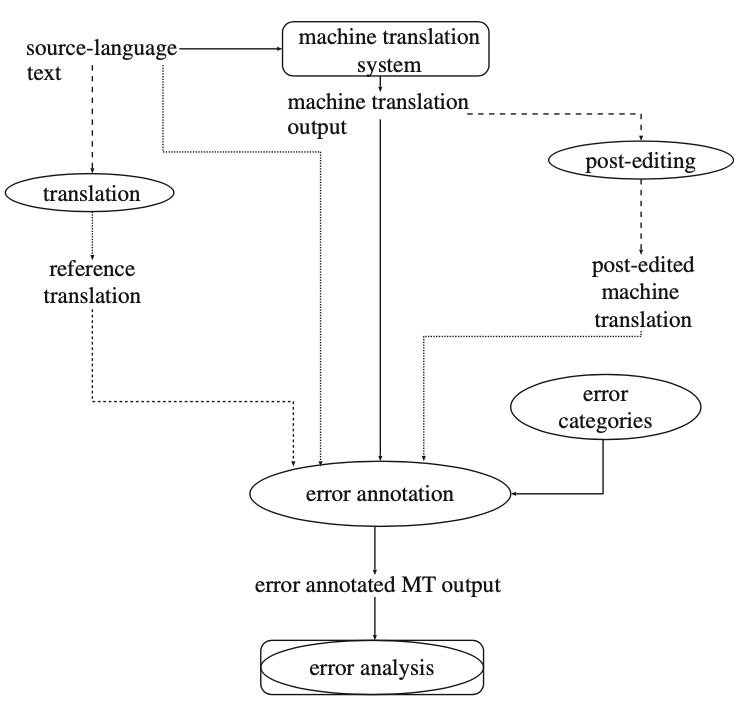
\includegraphics[width=0.7\textwidth]{textual/Figuras/human evaluation.png}
\caption{Manual Error Annotation: rectangles denote automatic processes and ellipses denote manual processes \parencite{popovic-2018}.} 
\label{fig: human-evaluation} 
\end{figure}

Frameworks like the Multidimensional Quality Metrics (MQM) offer an extensive list of error categories, which can be overwhelming \parencite{Mariana2014TheMQ}. A simpler approach, according to \textcite{Moorkens-2018}, is to use a limited set of common error types during evaluation, such as \emph{word order} mistakes (words not appearing in the correct order), \emph{mistranslations} (inaccurate or not fluent in the target language), \emph{omissions} (missing words from the source text), and \emph{additions} (words not found in the source text).

Once error categories are defined, applying them to real-world translations becomes crucial. However, as highlighted by~\textcite{Rossi2022}, it is important to note that a small sample of translated text might not be representative of an MT engine's overall performance. Ideally, human experts would evaluate multiple samples to choose the best system. But large-scale testing requires significant resources. Smaller enterprises might rely on automatic scoring, measuring the time and effort required to fix the translations (post-editing effort), or using a combination of both methods to ensure a more accurate assessment.


\subsection{Automatic Evaluation Metrics}

Automatic evaluation metrics (AEMs) offer a significant advantage over human assessment: they are considerably faster and more cost-effective. This advantage allows MT providers to perform frequent checks on the quality of their systems. According to~\textcite{Rossi2022}, AEMs are particularly useful in two key scenarios:

\begin{description}
    \item[MT Engine Development:] During the development of an MT engine, AEMs can be used to evaluate the engine's performance after each modification. This allows developers to determine if the changes have improved the engine's performance for their specific needs.
    \item[MT Option Selection:] When choosing an MT option for a project, AEMs can be employed to compare the quality of translations produced by different MT systems for the same source text. This comparison helps users select the most suitable MT system for their project requirements.
\end{description}

It is important to acknowledge that human translators often produce different, yet valid, translations for the same source text. As a result, we cannot expect an MT system to perfectly match a human translation. However, the closer a machine translation is to a human translation, the generally better it is considered to be \parencite{Rossi2022}. Many AEMs are built on this principle of similarity. These tools compare the MT output (called the \emph{candidate translation} or \emph{hypothesis}) to a human-generated ``gold standard'' or \emph{reference translation} to calculate scores. Some AEMs can even be incorporated with multiple reference translations to account for natural variations in human translation.

While AEMs are valuable for MT evaluation, \textcite{koehn2020neural} highlights a tension between the trust researchers place in these metrics and the ongoing debate about their true effectiveness in assessing MT quality. While AEMs heavily influence system design due to their focus on score optimization, researchers acknowledge their limitations and frequently challenge their validity. 


\subsubsection{Core concepts: \emph{n}-grams, precision, recall and F-measure}

This subsection introduces four core concepts: \emph{n}-grams, precision, recall, and F-measure, which form the building blocks of the more elaborate AEMs presented subsequently.

\subsubsection{\emph{n}-grams}

\emph{n}-grams, sequences of \emph{n} words, are a fundamental concept in many AEMs. In simpler terms, they represent groupings of consecutive words in a text. For instance, in the sentence ``He swam across the river,'' ``he'' is a unigram (1-gram), ``he swam'' is a bigram (2-gram), and ``he swam across'' is a trigram (3-gram). Similarly, 4-grams, 5-grams, and so on can be formed by extending the sequence length.

According to \textcite{Rossi2022}, \emph{n}-grams play a vital role in language modeling, where they estimate the probability of a word appearing based on the preceding \emph{n}-words. For example, in metrics such as BLEU, a trigram probability might indicate the likelihood of encountering a specific word given the two words before it in a sentence.

In the context of AEMs, \emph{n}-grams are typically sequences of \emph{n} words in the candidate translation that also exist in the reference translation. This essentially compares the overlap between the candidate translation and the human-generated ``gold standard'' translation. It is important to note that recent advancements have led to AEMs that consider character sequences instead of words. In these cases, \emph{n}-grams refer to sequences of \emph{n} characters rather than \emph{n} words.


\subsubsection{Precision and Recall}

Precision and recall are fundamental concepts in NLP. \textcite{Rossi2022} illustrate these concepts with a simple example. Imagine a teacher asks a student to name the days of the week in English. The student replies with ``Monday, Tuesday.'' This student provided two correct answers and no incorrect ones. \emph{Precision}, which measures the ratio of correct answers to the total number provided, would be a perfect score of 100\% (two out of two). However, from the teacher's perspective, the answer is incomplete. The teacher knows there are seven days in a week, and the student omitted five of them. This highlights the concept of \emph{recall}, which refers to the ratio of correct answers provided to the total number of correct answers possible (in the ideal response). In this case, the student's recall score would be two out of seven, which is roughly 29\%.

In the context of AEMs, precision focuses on the ratio of correct words in the candidate translation; that is, those that also appear in the reference translation, to the total number of words in the candidate translation. Mathematically, it can be expressed as:

\begin{equation}    
 \text{precision of \emph{C}} = \frac{\text{no. of correct words in \emph{C}}}{\text{no. of words in \emph{C}}} \hspace{1cm}
\end{equation}

where \emph{C} is the candidate translation.

Recall, on the other hand, focuses on the ratio of correct words in the candidate translation to the total number of words in the reference translation. It essentially measures how well the candidate translation captures everything from the reference. Mathematically:

\begin{equation}    
 \text{recall of \emph{C}} = \frac{\text{no. of correct words in \emph{C}}}{\text{no. of words in \emph{R}}} \hspace{1cm}
\end{equation}

where \emph{C} is the candidate translation, and \emph{R} is the reference translation.

\subsubsection{F-measure}

The example with the days of the week by~\textcite{Rossi2022} highlights the trade-off between precision and recall. To prioritize precision, the student could withhold further answers after ``Monday, Tuesday'' to avoid potential mistakes. Conversely, prioritizing recall might lead them to list numerous answers, hoping some are correct. For instance, they might reply with ``Monday, Tuesday, Wednesday, Thursday, Friday, Saturday, Sunday, January, February, March, April, May, June, July, August, September, October, November, December.'' While their recall would soar to 100\% (7 out of 7 correct days), precision would plummet below 37\% (7 correct answers out of 19 total). Neither strategy is ideal from the teacher's perspective.

The F-measure seeks to balance precision and recall by calculating their harmonic mean. Mathematically, it is defined as:

\begin{equation}
\text{F-measure} = 2 \times \frac{\text{precision} \times \text{recall}}{\text{precision} + \text{recall}}
\end{equation} \break

which can also be reformulated as:

\begin{equation}
\text{F-measure} = 2 \times \frac{\text{no. of correct words in \emph{C}}}{\text{no. of words in \emph{C}} + \text{no. of words in \emph{R}}}
\end{equation} \break


The F-measure penalizes extreme values in either precision or recall, favoring outputs that achieve a balance between the two. 


\subsubsection{BLEU}

Traditional evaluation methods like word error rate (common in speech recognition) struggle with correctly evaluating MT outputs. These methods miss the subjectivity of translation and the importance of word order in conveying meaning. To address these limitations, IBM’s BLEU (Bilingual Evaluation Understudy) was developed as a more comprehensive approach to automatic evaluation \parencite{papineni-etal-2002-bleu}

BLEU goes beyond simple word matching. It analyzes \emph{n}-grams (sequences of words up to 4 words long) in both the MT output and reference translations. By comparing the number of matching \emph{n}-grams and their order, BLEU rewards translations that preserve the original structure. Essentially, it is a precision metric focusing on the proportion of \emph{n}-grams in the MT output that also appear in the reference(s). The overall BLEU score is calculated as a geometric mean of individual \emph{n}-gram precisions  \parencite{koehn2020neural}.

While BLEU allows for multiple reference translations for flexibility, it emphasizes precision through a \emph{brevity penalty}. This discourages excessively short translations by penalizing outputs with a lower word count than the reference. The BLEU score itself is a combination of this penalty and a weighted sum of \emph{n}-gram precisions (ratio of matching n-grams in the machine translation to the reference(s)). Although using multiple references is less common now, it remains a valuable option.

The formula for BLEU, as defined in \textcite{koehn2020neural}, is presented below:

\begin{equation}
    \text{BLEU} = \text{BP} \times \exp \sum_{n=1}^{4} \log \left( \frac{\text{matching \emph{n}-grams}}{ \text{total \emph{n}-grams in machine translation}} \right) 
\end{equation}

\begin{equation}
    \text{BP} = \text{min} \left(1, \frac{\text{output-length}}{\text{reference-length}} \right)
\end{equation}

Here, BP represents the brevity penalty.

It is important to acknowledge that BLEU is a valuable tool, but not a perfect replacement for human evaluators. As highlighted in \textcite{koehn2020neural}, it has limitations:

\begin{description}
    \item[Ignores Word Importance:] 
    BLEU assigns equal weights to all words in a sentence, even though some words like ``not'' or proper nouns hold greater meaning compared to determiners (``the'', ``a'') or punctuation.
    \item[Overlooks Grammar:] BLEU focuses on matching \emph{n}-grams from the generated text to the references. This can lead to high scores for nonsensical sentences with the right \emph{n}-grams, but lacking overall grammatical correctness. 
    \item[Meaningless Scores:] BLEU scores are sensitive to factors like the number of reference translations, language pair, and even word segmentation. This makes interpreting scores (e.g., 30\%) and comparing translations across settings difficult.
    \item[Low Human BLEU Scores:] Experiments show that human translations compared against each other using BLEU still score relatively low. This suggests BLEU might not capture the full complexity of good human translation.
\end{description}


In essence, the critique argues that BLEU is a flawed metric because it does not reflect the true quality of an automatic translation. It might favor translations with matching \emph{n}-grams but poor grammar or miss important nuances that affect meaning.


\subsubsection{METEOR}

Evaluating MT accuracy often relies on surface-level comparisons between the candidate texts and human references. This approach can be misleading, as changes in wording or sentence order might not affect the core meaning. Simple evaluation metrics often penalize such variations, leading to inaccurate assessments \parencite{koehn2020neural}.

While traditional metrics like BLEU focus on surface-level \emph{n}-gram matching, METEOR tackles this limitation by incorporating semantics through stemming and synonyms. Stemming recognizes that words with the same root carry similar meaning (e.g., ``responsibility'' and ``responsible'' are both stemmed to ``respons''). METEOR also considers synonyms as valid matches, understanding that translators might choose ``security'' or ``safety,'' or ``responsibility'' or ``charge,'' without affecting the core meaning \parencite{koehn2020neural}. 

To evaluate a translation, METEOR employs a multi-step matching process, first attempting exact word matches and then considering stemmed forms or synonyms using WordNet synsets \parencite{saadany-orasan-2021-bleu, pedersen-etal-2004-wordnet}.

METEOR first calculates unigram precision and recall. Then, a harmonic mean (F-mean) is computed. This metric emphasizes recall, placing more weight on capturing all correct words from the reference:

\begin{equation}
\text{F-mean} =  \frac{10 \times (\text{precision} \times \text{recall})}{9 \times \text{recall} + \text{precision}}
\end{equation} 

While METEOR's core scoring focuses on unigram matches, it goes a step further by penalizing translations that significantly alter the word order. This discourages translations that capture meaning but severely mangle sentence structure \parencite{banerjee-lavie-2005-meteor}

METEOR assesses word order preservation by analyzing how well mapped words (between translation and reference) are grouped together. Ideally, these mapped words should appear consecutively in both texts (fewer chunks). The more scattered these mapped words are (more chunks), the higher the penalty. This penalty is calculated as:

\begin{equation}
\text{Penalty} = 0.5 \times \frac{\text{\# chunks}}{\text{\# unigrams-matched}}
\end{equation} 

For instance, with a candidate translation of ``the president spoke to the audience'' and a reference of ``the president then spoke to the audience,'' there are two chunks (``the president'' and ``spoke to the audience''), resulting in a penalty. The penalty increases with more chunks (up to a maximum of 0.5), and decreases with fewer chunks (minimum depends on matched unigrams) \parencite[68]{banerjee-lavie-2005-meteor}.

Finally, the METEOR score combines the F-mean and the penalty, with a higher penalty for poorer word order preservation. For multiple reference translations, METEOR picks the best score after evaluating against each. The overall system score is obtained by aggregating statistics across the entire test set.

\begin{equation}
\text{METEOR} = \text{F-mean} \times (1 - \text{Penalty})
\end{equation} 

While METEOR offers a more nuanced evaluation than BLEU, \textcite{koehn2020neural} emphasizes it comes with added complexity. METEOR requires resources like stemmers and synonym databases, which can be computationally expensive. The matching process involves aligning words between the MT output and the reference translation, adding further computational overhead. Additionally, METEOR has several parameters that need to be fine-tuned for optimal performance, such as the weight given to recall versus precision or the importance of stemming and synonym matches.

In essence, METEOR offers a more sophisticated approach to MT evaluation by considering semantic relationships between words. However, its increased complexity requires careful consideration of computational resources and parameter optimization.


\subsubsection{BERTScore}

Traditional metrics like BLEU and METEOR rely on \emph{n}-gram matching, focusing on surface-level similarities between the candidate text and a reference. This approach often disregards the deeper meaning, particularly when it comes to paraphrases. For example, as \textcite{saadany-orasan-2021-bleu} point out, these metrics might score ``people like visiting places abroad'' higher than ``consumers prefer imported cars,'' even though both may convey the same preference for foreign things in different words.

Newer approaches address this limitation by leveraging pre-trained language models like BERT. BERTscore \parencite{zhang2020bertscore} exemplifies this approach. It calculates a score based on the similarity in contextual meaning between each word in the translation and the reference. By using contextual embeddings, similar to how humans understand language, BERTScore captures the meaning of each word in relation to others. This allows it to accurately assess paraphrases and even distant dependencies in word order, such as the difference between ``A because B'' and ``B because A.'' These capabilities lead to a more accurate and comprehensive evaluation that considers both meaning and structure.

BERTScore evaluates the similarity between a reference (denoted by $x = ⟨x_1, ..., x_k⟩$) and a candidate (denoted by $\hat{x} = ⟨\hat{x}_1, ..., \hat{x}_l⟩$) using contextual embeddings and cosine similarity. These embeddings capture the meaning of each word based on its surrounding context. Figure~\ref{fig: bertscore} illustrates the computation. Optionally, inverse document frequency (idf) scores can be incorporated to emphasize the importance of rare words.

\begin{figure}[htb]
\centering
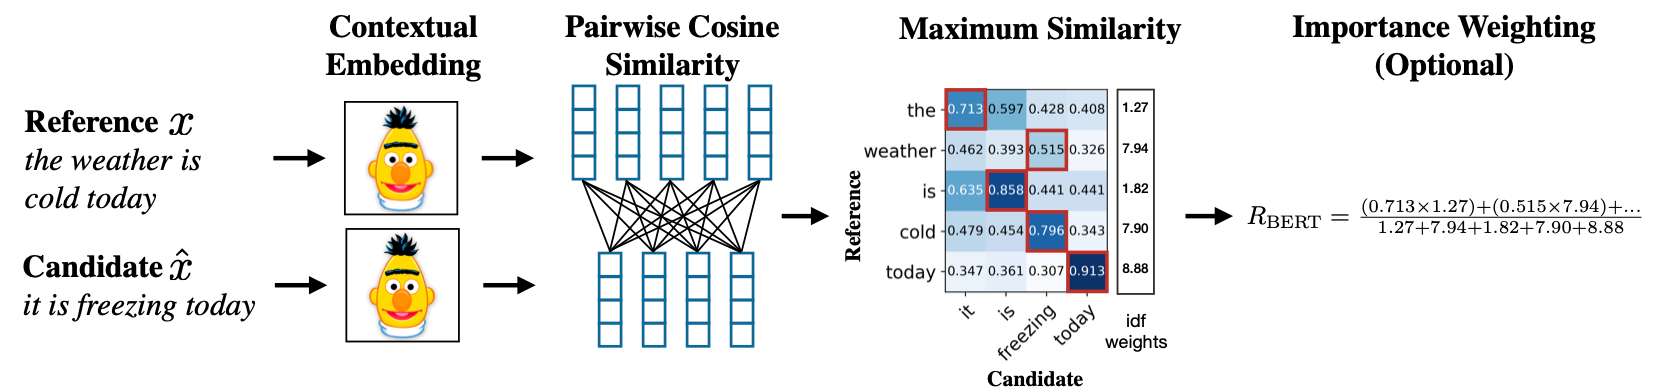
\includegraphics[width=1\textwidth]{textual/Figuras/bertscore.png}
\caption{BERTScore Recall ($R_{BERT}$) computation. Shows BERT embeddings, cosine similarity for all word pairs (lines), greedy matching (red arrows), and optional idf weighting \parencite{zhang2020bertscore}.} 
\label{fig: bertscore} 
\end{figure}

Key Components of BERTScore \parencite{zhang2020bertscore}:

\begin{description}
    \item[Contextual Embeddings:] To generate contextual embeddings, BERTScore utilizes models like BERT \parencite{devlin-etal-2019-bert} or ELMO \parencite{peters-etal-2018-deep} to represent tokens in the input sentences $x$ (reference) and $\hat{x}$ (candidate). These embeddings use vector representations to capture the meaning of a word based on its surrounding context, allowing for more nuanced comparisons than traditional word embeddings that only consider the word itself.
    \item[Similarity Measure:] Instead of exact string matching, BERTScore employs cosine similarity to measure the similarity between a reference and a candidate sentence. Cosine similarity calculates the angle between two vectors, with a higher value indicating greater similarity. In BERTScore, the cosine similarity of a reference token $x_i$ and a candidate token $\hat{x}_j$ is is calculated is calculated using their pre-normalized embedding vectors: $x_i \boldsymbol{\top} \hat{x}_j$. While this measure considers tokens in isolation, the contextual embeddings inherently contain information about the surrounding context, allowing for scoring even when paraphrases or different word choices are used.
    \item[Greedy Matching:] BERTScore uses greedy matching to find the most similar word in the candidate sentence ($\hat{x}_j$) for each word in the reference sentence ($x_i$). This matching helps calculate two key metrics: recall and precision. Recall measures how well it finds all the words from the reference sentence in the candidate sentence. Precision measures how accurate those matches are (avoiding extra, irrelevant words in the candidate sentence). Recall and precision are calculated as shown in Equations~\ref{r-p-bert}.
\end{description}

    \begin{equation} \label{r-p-bert}
    R_{BERT} = \frac{1}{|x|} \sum_{x_i∈x} \max_{\hat{x}_j∈\hat{x}} \left(\boldsymbol{x}_i \top \hat{\boldsymbol{x}}_j \right),
     P_{BERT} = \frac{1}{|\hat{x}|} \sum_{\hat{x}_i∈\hat{x}} \max_{x_j∈x} \left( \boldsymbol{x}_i \top \hat{\boldsymbol{x}}_j \right) \\
    \end{equation}
    
\begin{description}       
    \item[F1 Score:] BERTScore combines precision (percentage of relevant tokens matched) and recall (percentage of reference tokens found) to create an F1 score, providing a balanced measure of performance. F1 score is calculated as in Equation~\ref{f-bert}.
\end{description} 

    \begin{equation} \label{f-bert}
    F_{BERT} = 2 \times \frac{P_{BERT} \cdot R_{BERT}}{P_{BERT} + R_{BERT}}
    \end{equation}
    
\begin{description}     
    \item[Importance Weighting (Optional)]: BERTScore can optionally incorporate inverse document frequency ($idf$) scores to emphasize the importance of rare words in determining sentence similarity. Given $M$ reference sentences $\left\{{x^{(i)}} \right\}_{i=1}^{M}$, the idf score of a word-piece token $w$ is defined by Equation~\ref{idf}.
\end{description} 

    \begin{equation} \label{idf}
    idf(w) = - \log \frac{1}{M} \sum_{i=1}^{M} \mathds{1} [w∈x^{(i)}],
    \end{equation}

\begin{description}    
    \item[\hspace{=2em}]where, $\mathds{1}[\cdot]$ is an indicator function. The full $td-idf$ measure is not used because single sentences are processed, where the term frequency ($tf$) is likely 1. For example, recall with $idf$ weighting is as in Equation~\ref{r-bert-idf}:
\end{description}

    \begin{equation} \label{r-bert-idf}
     R_{BERT} = \frac{\sum_{x_i \in x} \text{idf}(x_i) \max_{\hat{x}_j \in \hat{x}} \left( \boldsymbol{x}_i \top \hat{\boldsymbol{x}}_j \right) }{\sum_{x_i \in x} \text{idf}(x_i)} \\
    \end{equation}
    
\begin{description}    
    \item[\hspace{=2em}]Because references are used to compute idf, the scores remain the same for all systems evaluated on a specific test set. Then, plus-one smoothing is applied to handle unknown word pieces.
\end{description}
    
\begin{description}    
    \item[Baseline Rescaling:] Pre-normalized vectors are used, so computed scores have the same numerical range of cosine similarity (between −1 and 1). However, to improve readability, BERTScore rescales its scores to a range between 0 and 1, considering the typical score distribution for low-similarity sentence pairs, using Equation~\ref{r-bert-baseline}.
\end{description}    

    \begin{equation} \label{r-bert-baseline}
     \hat{R}_{BERT} = \frac{R_{BERT} - b}{1 − b}
    \end{equation}

\begin{description}    
    \item[\hspace{=2em}]After applying the formula, $\hat{R}_{BERT}$ is typically between $0$ and $1$. The same rescaling procedure is done with $\hat{P}_{BERT}$ and $\hat{F}_{BERT}$.
\end{description}    


Despite outperforming \emph{n}-gram based BLEU in many scenarios, BERTScore's effectiveness can vary depending on specific elements within the text, particularly function words, as discussed by~\textcite{hanna-bojar-2021-fine}. This leads it to struggle with slight phrasing variations, such as tag questions (e.g., ``You're crazy, aren't you?'') and other nuanced linguistic features. Furthermore, BERT-based metrics like BERTScore have difficulty differentiating between incorrect translations that closely resemble the reference and more accurate ones with different wording, especially when stylistically similar.

Adding to these limitations, \textcite{sun-etal-2022-bertscore} identified a concerning bias (i.e., race, gender, religion, physical appearance, age, and socioeconomic status) in pre-trained metrics like BERTScore. These metrics exhibit significantly higher bias on sensitive attributes like gender compared to traditional \emph{n}-gram based metrics. For example, gender bias resulted in score differences of $7$-$21$ points for BERT-based metrics, whereas traditional metrics showed minimal bias ($< 1.3$ points). This might be due to how datasets are constructed for evaluation, inadvertently including stereotypes present in source data.


\subsubsection{COMET}

The recent surge in research on using neural networks to train MT models has led to significant improvements in MT quality. However, evaluating these systems has not kept pace. As pointed out by \textcite{ma-etal-2019-results, rei-etal-2020-comet}, existing AEMs still have weaknesses. For example, they might disagree with human judgments on individual sentences and struggle to distinguish between the very best performing MT systems.

COMET (Crosslingual Optimized Metric for Evaluation of Translation) \parencite{rei-etal-2020-comet}, offers a new approach to MT evaluation. This framework, built with PyTorch, trains multilingual models to assess translation quality. Inspired by recent work in Quality Estimation (QE) that showed promise in evaluating translations without a perfect reference, COMET incorporates the source language text itself. This approach differs from traditional AEMs, which typically rely solely on a reference translation for comparison.

COMET offers two distinct model architectures, as illustrated in Figure\ref{fig: comet}, to address different aspects of MT evaluation:

\begin{figure}[htb]
\centering
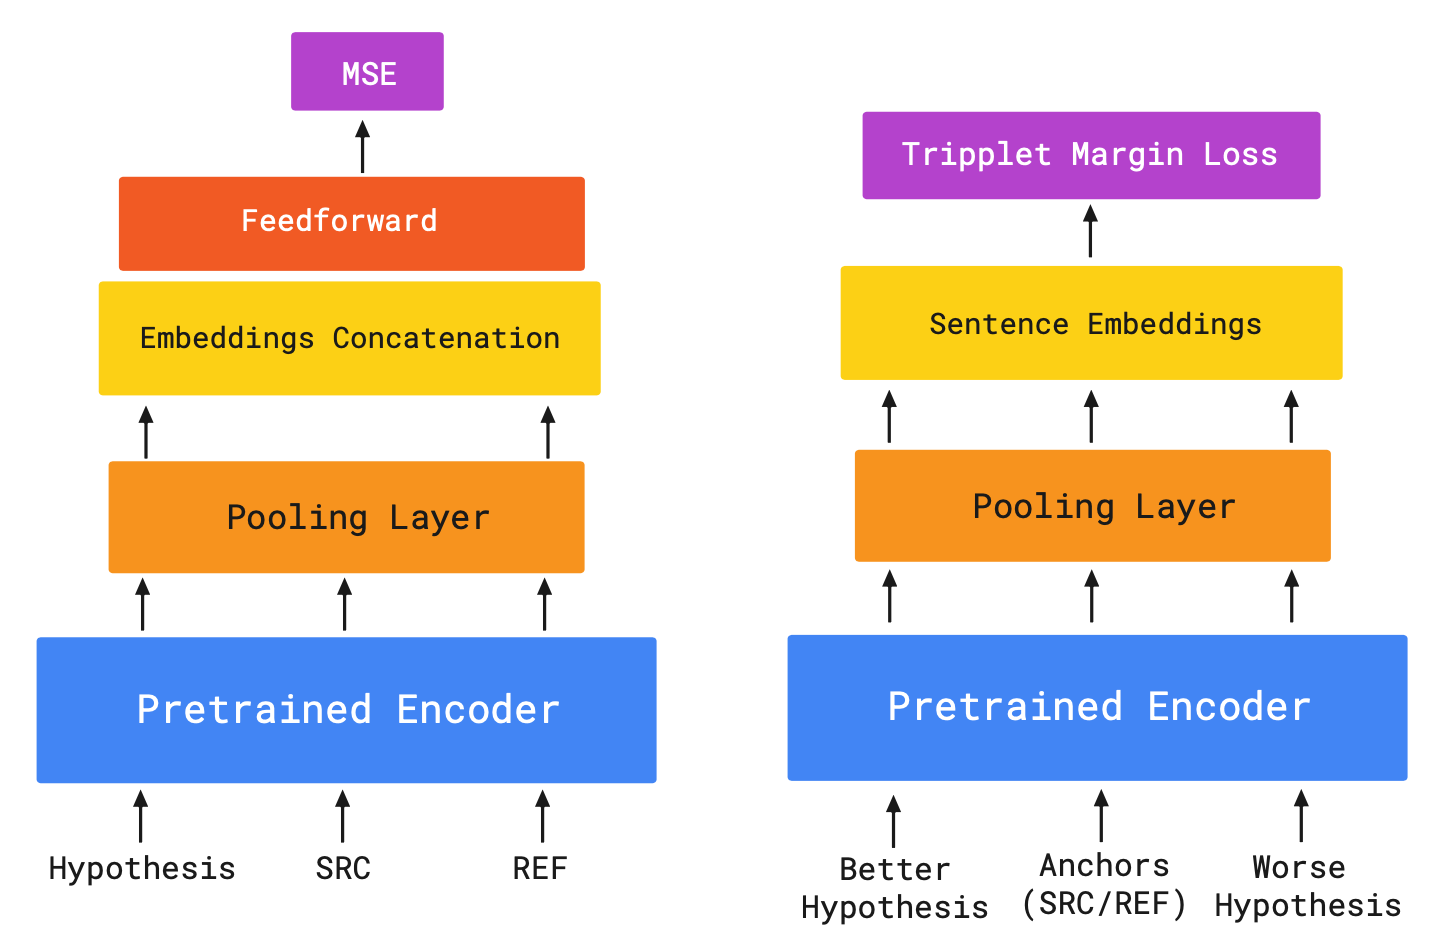
\includegraphics[width=.8\textwidth]{textual/Figuras/comett.png}
\caption{Estimator Model (left): Analyzes source text, translated text (hypothesis), and reference (optional) using a multilingual encoder. It captures the essence of each sentence (embedding) and combines this information (if a reference exists) through concatenation. Finally, it learns from human quality ratings (DA, HTER, or MQM) to predict a score for the translation via a feed-forward regressor, minimizing the Mean Squared Error (MSE). Translation Ranking Model (right): Focuses on relative quality comparison between translations of the same source text. Similar to the Estimator model, it analyzes them using a multilingual encoder to generate embeddings. During training, the model utilizes triplet margin loss to position these embeddings in the embedding space. The ``better'' translation's embedding should be closer to both the source text and the reference (if available) compared to the ``worse'' translation's embedding. This helps COMET distinguish high-quality translations \parencite{rei-etal-2020-comet}.}


\label{fig: comet} 
\end{figure}

\begin{description}    
    \item[Estimator model] (Figure\ref{fig: comet} -- on the left): This model is directly trained to predict a quality score for a given translation.
    \begin{description}
        \item \emph{Cross-lingual Encoder}: This is the foundation of both models. It utilizes a pretrained, cross-lingual model like multilingual BERT \parencite{devlin-etal-2019-bert}, with multiple transformer encoder layers, to analyze the source text, translated text (hypothesis), and reference translation (if available). The encoder considers the relationships between words within each text.
        \item\emph{Pooling Layer}: This layer combines the information from each word embedding generated by the encoder, not just the last one, to create a single embedding for each sentence. This is shown to increase model performance on MT evaluation tasks \parencite{zhang2020bertscore}. This embedding is computed as in Equation~\ref{embeding}:
            \begin{equation} \label{embeding}
            \mathbf{e}_{x_j} = \mu \mathbf{E}_{x_j}^\top \boldsymbol{\alpha}
            \end{equation}
        where, $\mathbf{e}_{x_j}$ is the embedding vector for token x, $\mu$ is the weight coefficient (scalar), $\mathbf{E}_{x_j}$ is the matrix containing layer embeddings for token x (j-th row corresponds to layer l) and $\alpha$ is the trainable weight vector corresponding to layer-wise importance (one weight per layer).
        \item\emph{Embedding Concatenation}: When the Estimator model has a reference translation, it creates embeddings for the source text, hypothesis, and reference. Concatenation simply combines these embeddings into a single list, allowing the model to consider all the information together.
        \item\emph{Feed-forward Regressor}: The sentence embeddings from the source, hypothesis, and reference (if available) are combined and fed into this layer. The regressor is trained to minimize the Mean Squared Error (MSE) between the predicted scores and human quality assessments (DA, HTER, or MQM).
    \end{description}
    \item[Translation Ranking model] (Figure\ref{fig: comet} -- on the right): focuses on learning the relative quality between different translations for the same source text. 
    \begin{description}
        \item\emph{Similar to the Estimator model}: This model also utilizes a cross-lingual encoder and pooling layer to generate sentence embeddings.
        \item\emph{Triplet Margin Loss}: During training, the model is presented with three translations for the same source text: a ``better'' translation, a ``worse'' translation, and optionally, a reference translation. Triplet margin loss encourages the model to position these embeddings in a way that reflects their quality. Ideally, the ``better'' translation's embedding should be closer to both the source text and the reference translation (if available) compared to the ``worse'' translation's embedding. This helps the model learn to distinguish between higher and lower quality translations.
    \end{description}
\end{description}

While COMET has proven effective in translation evaluation, it is not without limitations. Studies by \textcite{glushkova2023bleu} highlight specific error types that COMET struggles with. These include discrepancies in numbers between the source text and translation, mistranslated or missing named entities, unintended omissions of important content, and unnecessary insertions of words not present in the original text. These challenges have been echoed in other research \parencite{amrhein-sennrich-2022-identifying, alves-etal-2022-robust}. Attempts to address these issues using data augmentation techniques have shown some improvement \parencite{alves-etal-2022-robust}, but the gains appear to be modest.


\subsubsection{TER}

The translation error rate (TER), also known as translation edit rate, is a metric that goes beyond simple word-level accuracy and takes into account the order of words in a sentence. It builds upon the concept of word error rate (WER), a metric borrowed from speech recognition, which leverages the \emph{Levenshtein distance} to determine the minimum number of editing steps (insertions, deletions, substitutions) needed to transform one sequence of words into another \parencite{snover-etal-2006-study, koehn2012statistical}.

The Levenshtein distance can be thought of as measure of editing effort. WER takes this effort and compares it to the length of the correct translation (reference). This gives us an error rate as a percentage. A perfect translation scores 0\%, while a completely scrambled sentence scores 100\%.

Mathematically, the formula for WER is:

\begin{equation}
\text{WER} = \frac{\text{substitutions} + \text{insertions} + \text{deletions}}{\text{reference-length}}
\end{equation} 

Here, ``reference-length'' is the number of words in the reference translation.

WER treats each word move (or where a sequence of words is shifted elsewhere in the sentence) as two errors (one deletion and one insertion). This can lead to an inflated error rate for translations where the overall meaning is preserved but word order is shuffled \parencite{Rossi2022}.

TER addresses this limitation by introducing a ``shift'' operation. This means that moving any sequence of words counts as only one error, providing a more accurate reflection of errors that impact meaning:

\begin{equation}
\text{TER} = \frac{\text{shifts} + \text{substitutions} + \text{insertions} + \text{deletions}}{\text{reference-length}}
\end{equation} 

\textcite{koehn2020neural} highlights a major issue with using WER for MT. Here is an example:

\begin{boxK}
    \textbf{Hypothesis}: A spokesperson announced today: “The plan will go forward.” \\
    \textbf{Reference}: “The plan will go forward,” a spokesperson announced today.
\end{boxK}

WER harshly penalizes reordered sentences by treating the movement of the entire main clause (``A spokesperson announced today'') as separate deletion (4 errors) and insertion (another 4 errors) for a 9-word sentence, leading to an excessively inflated error rate. In contrast, TER considers such movement a single shift'' error, resulting in a much more accurate and reasonable score of just 1/9 ≈ 11\% for our example.

TER scores are not only easier to understand but also a superior metric for evaluating individual sentences. BLEU score calculation involves 4-gram precision, but a translated sentence might lack any matching 4-grams, leading to a BLEU score of 0. While TER is not as widely adopted as BLEU, it is a more suitable option for sentence-level evaluation.

Algorithm~\ref{alg:ter} calculates the minimum number of edits (shifts, substitutions, insertions, and deletions) required to transform a translated sentence (hypothesis) into a correct reference sentence as in~\textcite{snover-etal-2006-study}.

\bigskip 

\begin{algorithm}
\small
\caption{Calculate Number of Edits}\label{alg:ter}
\hspace*{\algorithmicindent} \textbf{Input:} HYPOTHESIS $h$ \\ 
\hspace*{\algorithmicindent} \textbf{Input:} REFERENCES $R$
\begin{algorithmic}
\State $E\gets∞$ \Comment{Initialize minimum edits}
\For{$r∈R$}
\State $h\gets h$ \Comment{Copy hypothesis}
\State $e\gets0$ \Comment{Initialize edit count}
\Repeat
\State Find shift, $s$, that most reduces min-edit-distance$(h′, r)$
\If{$s$ reduces edit distance}
\State $h′\gets$ apply $s$ to $h′$ 
\State $e\gets e+1$
\EndIf
\Until{No shifts that reduce edit distance remain}
\State $e\gets e+$ min-edit-distance$(h′, r)$
\If{$e<E$}
\State $E\gets e$
\EndIf
\EndFor
\State \textbf{return} $E$
\end{algorithmic}
\end{algorithm}

\bigskip 

To speed up finding good shifts (optimal edits are computationally expensive), a greedy search with specific rules is used \parencite{snover-etal-2006-study}. These rules prioritize shifts that improve accuracy: 1) shifted words must match the reference, 2) the source must differ from the reference, and 3) the destination must be initially misaligned.

\vspace{0.5em} % Adjust the value (e.g., 1em) to increase or decrease the gap

All in all, in Section~\ref{chap: tqa}, we explored various AEMs, from more traditional metrics like BLEU and METEOR to advanced ones like COMET and BERTScore. The comparative analysis highlights the strengths and limitations of each method, especially in handling linguistic nuances and ensuring accurate assessments. Moving forward, these insights are crucial for discussing MT effectiveness and guiding future advancements in translation quality estimation, providing a foundation for addressing challenges and opportunities in evolving MT technologies.
}
}